\documentclass[11pt,a4paper]{article}

\usepackage{iftex}
\ifPDFTeX
  \usepackage[utf8]{inputenc}
  \usepackage[T5,T1]{fontenc}
\else
  \usepackage{fontspec}
\fi
\usepackage[vietnamese,english]{babel}
\usepackage[a4paper,top=20mm,bottom=20mm,left=25mm,right=20mm]{geometry}

\usepackage{amsmath,amssymb,amsfonts}
\usepackage{booktabs}
\usepackage{tabularx}
\usepackage{graphicx}
\usepackage{caption,subcaption}
\usepackage{enumitem}
\usepackage{xcolor}
\usepackage{titlesec}
\usepackage{float}
\usepackage{algorithm}
\usepackage{algpseudocode}
\usepackage{setspace}

\usepackage[
    colorlinks=true,
    linkcolor=blue,
    citecolor=blue,
    urlcolor=blue
]{hyperref}

\onehalfspacing
\setlength{\parindent}{0pt}
\setlength{\parskip}{1.2ex}

\titlespacing*{\section}{0pt}{12pt}{6pt}
\titlespacing*{\subsection}{0pt}{10pt}{4pt}

\titleformat{\section}{\large\bfseries}{\thesection.}{0.5em}{}
\titleformat{\subsection}{\normalsize\bfseries}{\thesubsection.}{0.5em}{}

\renewcommand{\topfraction}{0.9}
\renewcommand{\bottomfraction}{0.8}
\renewcommand{\textfraction}{0.05}
\renewcommand{\floatpagefraction}{0.85}

\begin{document}
\selectlanguage{vietnamese}

\begin{center}
    {\Large\bfseries BÁO CÁO TIẾN ĐỘ THỰC HIỆN KHÓA LUẬN TỐT NGHIỆP}
\end{center}

\vspace{0.4cm}
\section{Nội dung đề tài và Mục tiêu nghiên cứu}

\subsection{Vấn đề thực tiễn và Động lực nghiên cứu}
Trong các mạng diện rộng (WAN) kết nối nhiều trung tâm dữ liệu và các hệ thống tự trị (ASes), việc tối ưu hóa định tuyến lưu lượng (Traffic Engineering - TE) là nhiệm vụ then chốt để duy trì chất lượng dịch vụ (QoS). Tuy nhiên, các giải pháp hiện nay đang đối mặt với ba hạn chế chính:
\begin{enumerate}[leftmargin=1.5em, itemsep=0.2ex]
    \item Định tuyến truyền thống mang tính bị động: Các giao thức như OSPF hay ECMP chỉ dựa trên độ dài đường truyền tĩnh. Khi xuất hiện các luồng dữ liệu lớn (Elephant Flows), hệ thống không dự báo trước được nguy cơ, dẫn đến nghẽn liên kết, đầy hàng đợi (Buffer Bloat), tăng trễ và mất gói.
    \item Rào cản chia sẻ dữ liệu giữa các miền mạng: Để dự báo lưu lượng toàn mạng, các phương pháp học máy tập trung đòi hỏi các miền mạng con phải gửi ma trận lưu lượng thô về máy chủ trung tâm. Điều này vi phạm chính sách bảo mật dữ liệu khách hàng và bí mật kinh doanh giữa các nhà cung cấp dịch vụ (ISPs).
    \item Hạn chế của DRL phản xạ tức thời: Các mô hình học tăng cường sâu (DRL) thông thường chỉ nhìn vào trạng thái tức thời nên phản ứng chậm (chỉ đổi đường sau khi đã nghẽn). Ngoài ra, tác tử không có bộ nhớ ngữ cảnh dễ bị đổi tuyến liên tục (Route Flapping) khi tải dao động nhẹ, làm xáo trộn thứ tự gói tin và giảm tốc độ truyền TCP.
\end{enumerate}

\subsection{Mục tiêu nghiên cứu}
Đề tài tập trung giải quyết các hạn chế trên thông qua bốn mục tiêu cụ thể:
\begin{itemize}[leftmargin=1.5em, itemsep=0.3ex]
    \item Dự báo tải liên kết bảo toàn quyền riêng tư đa miền: Xây dựng mô hình học liên kết (Federated Learning) kết hợp \texttt{TrafficLSTM} và thuật toán \texttt{FedAdam}. Các miền mạng hợp tác huấn luyện để dự báo tải liên kết trong 45 phút tới với sai số $\text{MAE} < 0.05$ mà không cần chia sẻ dữ liệu lưu lượng thô.
    \item Điều phối lưu lượng chủ động theo vòng lặp kín: Đưa vector tải dự báo tương lai $\mathbf{\hat{u}}_{t+1}$ vào trạng thái của tác tử \texttt{RecurrentPPO}, giúp tác tử chủ động phân bổ lại các luồng lớn sang đường phụ ($K$-Shortest Paths) trước khi liên kết chính bị nghẽn.
    \item Đảm bảo tính ổn định và an toàn định tuyến: Tích hợp tầng nhớ LSTM vào mạng chính sách để tạo quán tính hành động, triệt tiêu hiện tượng rung giật tuyến (giữ tỷ lệ đổi tuyến $\text{Churn} < 0.1\%$). Đồng thời triển khai rào chắn an toàn kiểm tra tải dự phóng để ngăn các quyết định chuyển luồng gây nguy cơ nghẽn.
    \item Đánh giá khả năng chuyển giao đa topo: Kiểm thử khả năng chuyển giao không mẫu (Zero-Shot) và tinh chỉnh nhanh (Fine-Tuning) của mô hình huấn luyện từ mạng GÉANT sang các topo mạng khác biệt như NSFNET và Abilene.
\end{itemize}

\section{Các nội dung đã thực hiện}

\subsection{Xây dựng mô hình mô phỏng mạng và trực quan hóa các Topo}
Hệ thống đã chuẩn hóa và cấu hình mô hình mạng hoàn chỉnh trên cả ba topo thực tế chuẩn quốc tế:
\begin{itemize}[leftmargin=1.5em, itemsep=0.2ex]
    \item NSFNET: Gồm 14 router, 42 liên kết có hướng, băng thông chuẩn 1 Gbps, độ trễ lan truyền 2--10 ms. Mạng được chia thành 3 miền: miền Tây (Domain A), miền Trung (Domain B) và miền Đông (Domain C).
    \item GÉANT: Cấu trúc dạng lưới dày gồm 22 router, 72 liên kết có hướng, băng thông 2.5 Gbps, độ trễ 1--15 ms. Mạng chia thành 3 miền: Bắc Âu (Domain A), Trung Âu (Domain B) và Nam Âu (Domain C).
    \item Abilene: Cấu trúc vành đai thưa gồm 12 router, 30 liên kết có hướng, băng thông 1 Gbps, độ trễ 2--15 ms giữa bờ Đông và bờ Tây Hoa Kỳ.
\end{itemize}

Đặc tính cấu trúc và thông số kỹ thuật của ba mô hình mạng được tổng hợp tại Bảng \ref{tab:topo_characteristics}, và kiến trúc triển khai phân miền được trực quan hóa tại Hình \ref{fig:topo_deployments}.

\begin{table}[H]
\centering
\caption{\textit{Bảng đối sánh đặc tính cấu trúc của ba mô hình mạng thực nghiệm.}}
\label{tab:topo_characteristics}
\footnotesize
\renewcommand{\arraystretch}{1.0}
\begin{tabularx}{\textwidth}{@{} l c c c c c X @{}}
\toprule
\textbf{Topo Mạng} & \textbf{Số nút ($|V|$)} & \textbf{Liên kết ($|\mathcal{E}|$)} & \textbf{Bậc TB} & \textbf{Dung lượng} & \textbf{Luồng Quản lý} & \textbf{Cấu trúc Hình học} \\
\midrule
NSFNET & 14 & 42 & 3.00 & 1.0 Gbps & 20 luồng voi & Dạng lưới thưa liên vùng (USA Mesh). \\
GÉANT & 22 & 72 & 3.27 & 2.5 Gbps & 30 luồng voi & Dạng lưới dày đa kết nối (EU Mesh). \\
Abilene & 12 & 30 & 2.50 & 1.0 Gbps & 15 luồng voi & Dạng vành đai thưa xuyên bờ (US Ring). \\
\bottomrule
\end{tabularx}
\end{table}

\begin{figure}[htbp]
    \centering
    \begin{subfigure}[b]{0.32\textwidth}
        \centering
        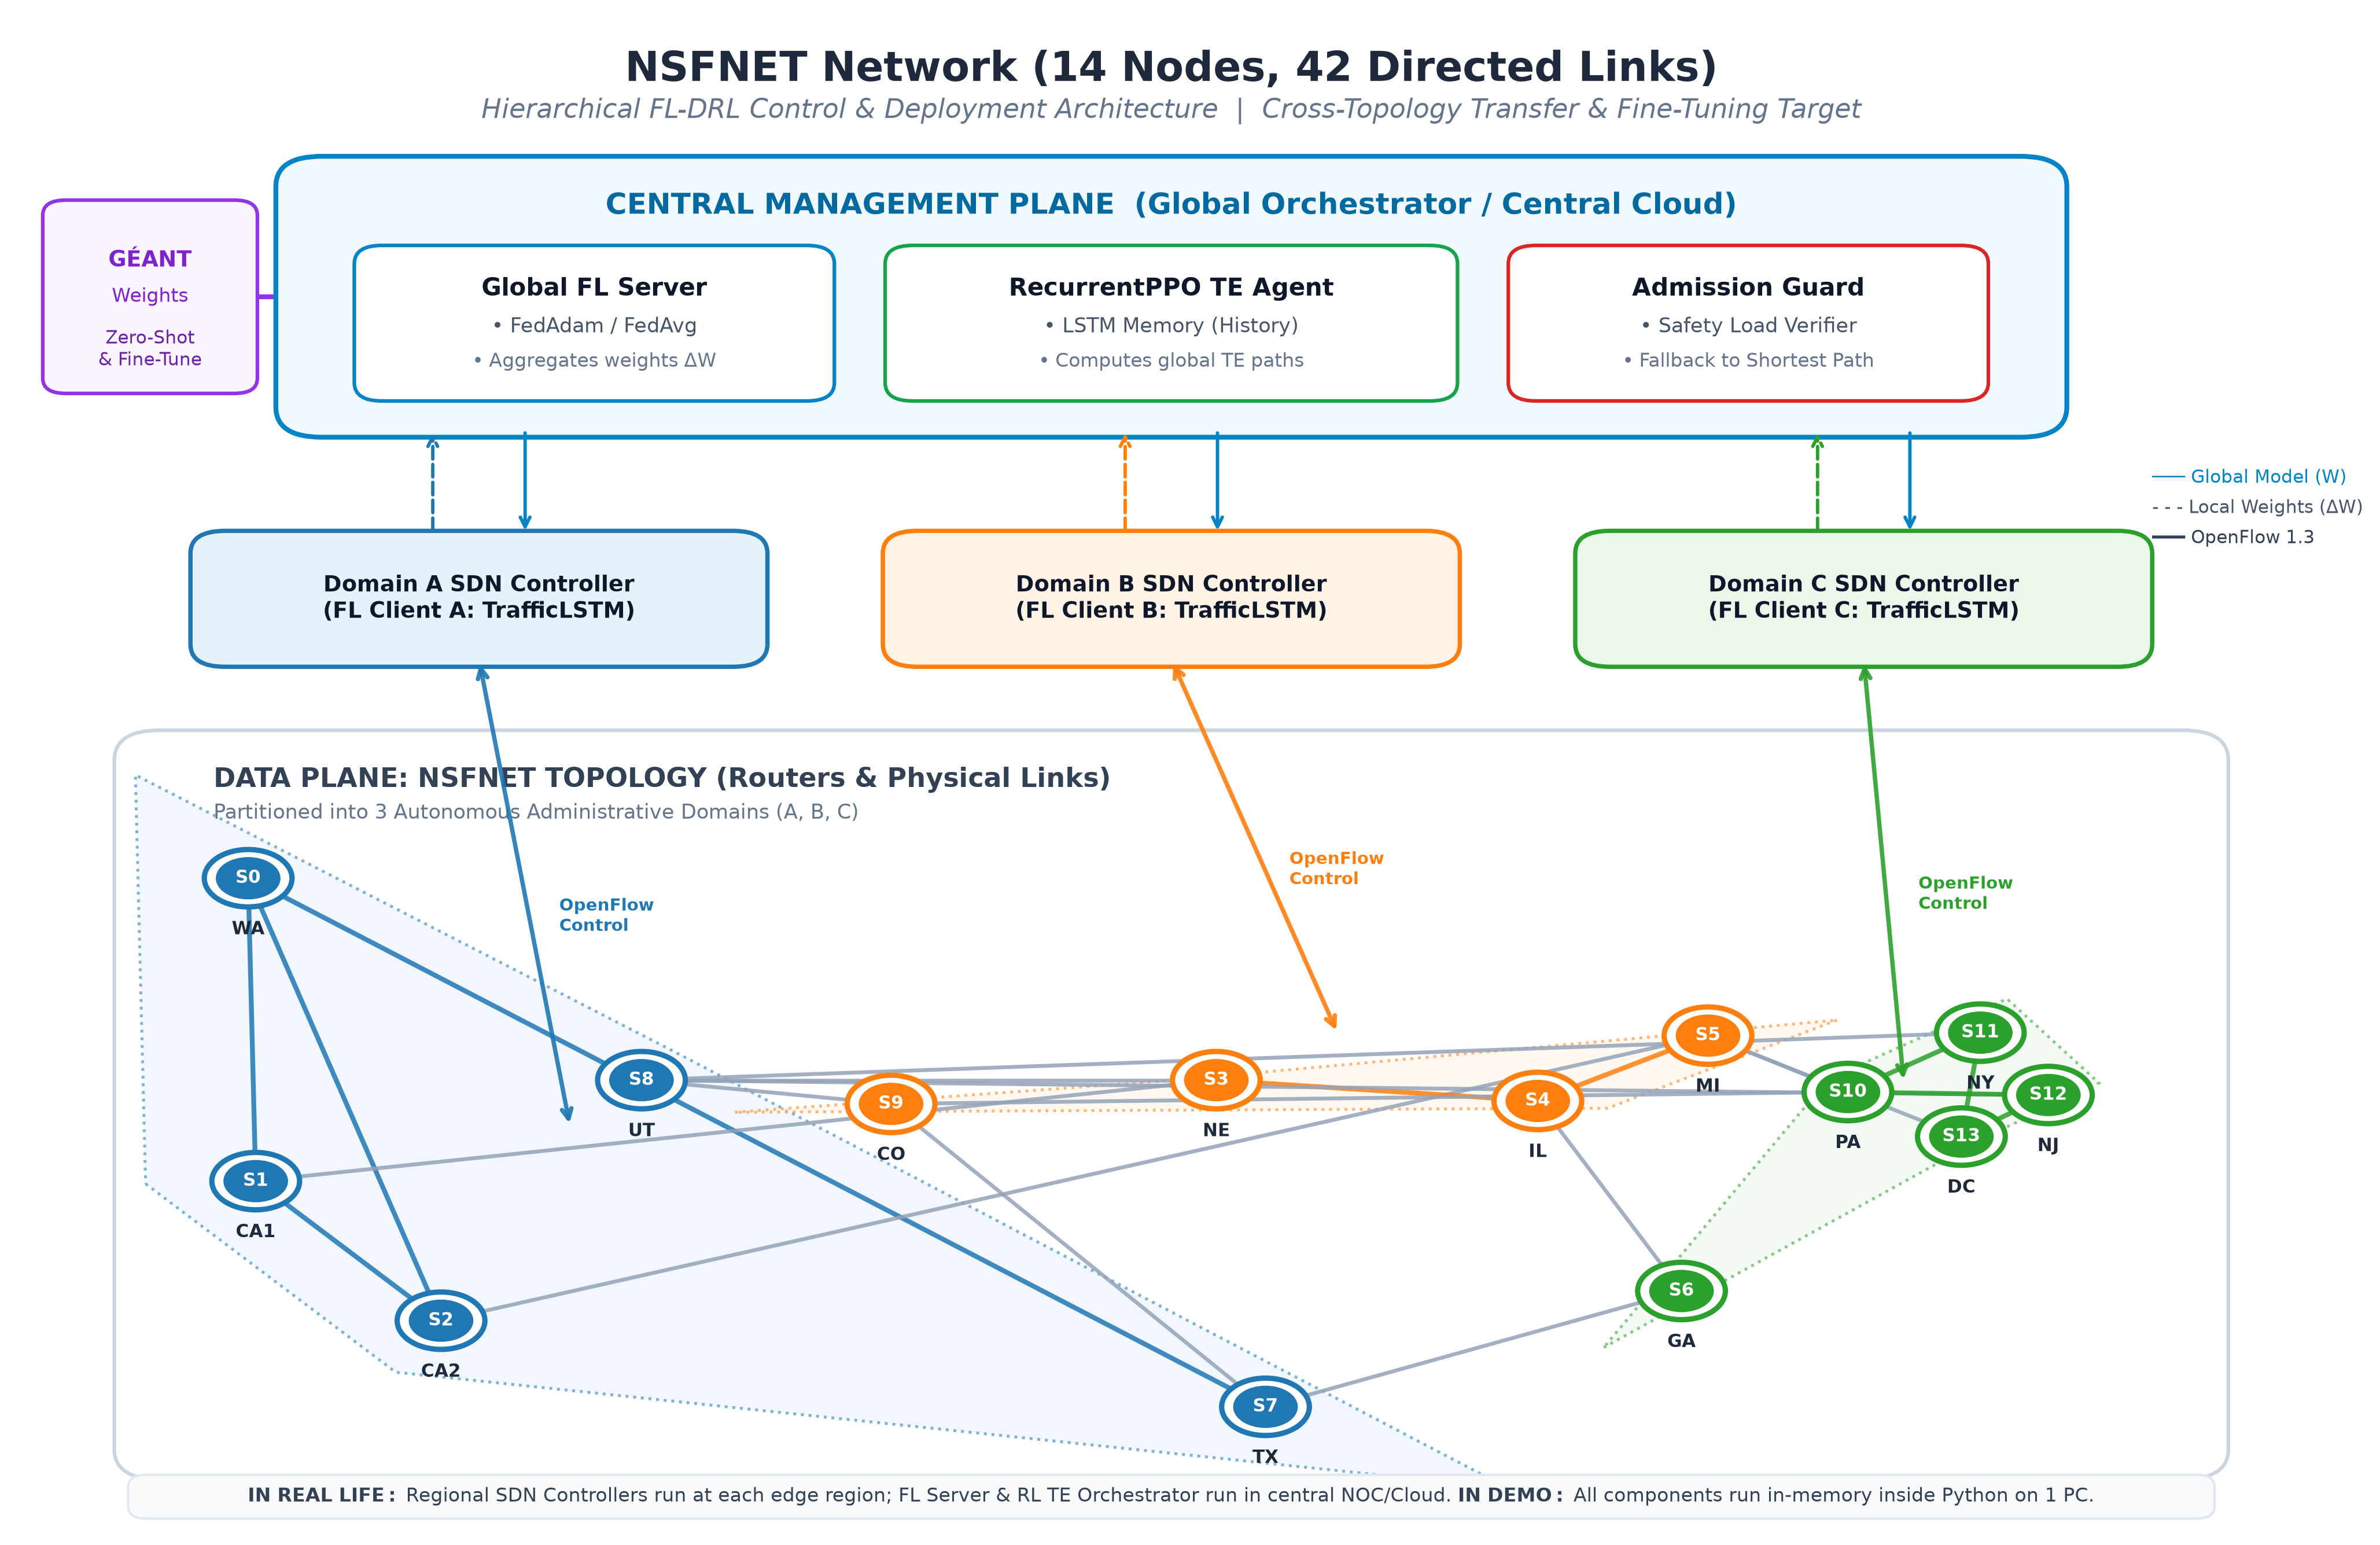
\includegraphics[width=\textwidth]{figures/topology_deployment_nsfnet.png}
        \caption{NSFNET (14 nút, 42 liên kết)}
    \end{subfigure}\hfill
    \begin{subfigure}[b]{0.32\textwidth}
        \centering
        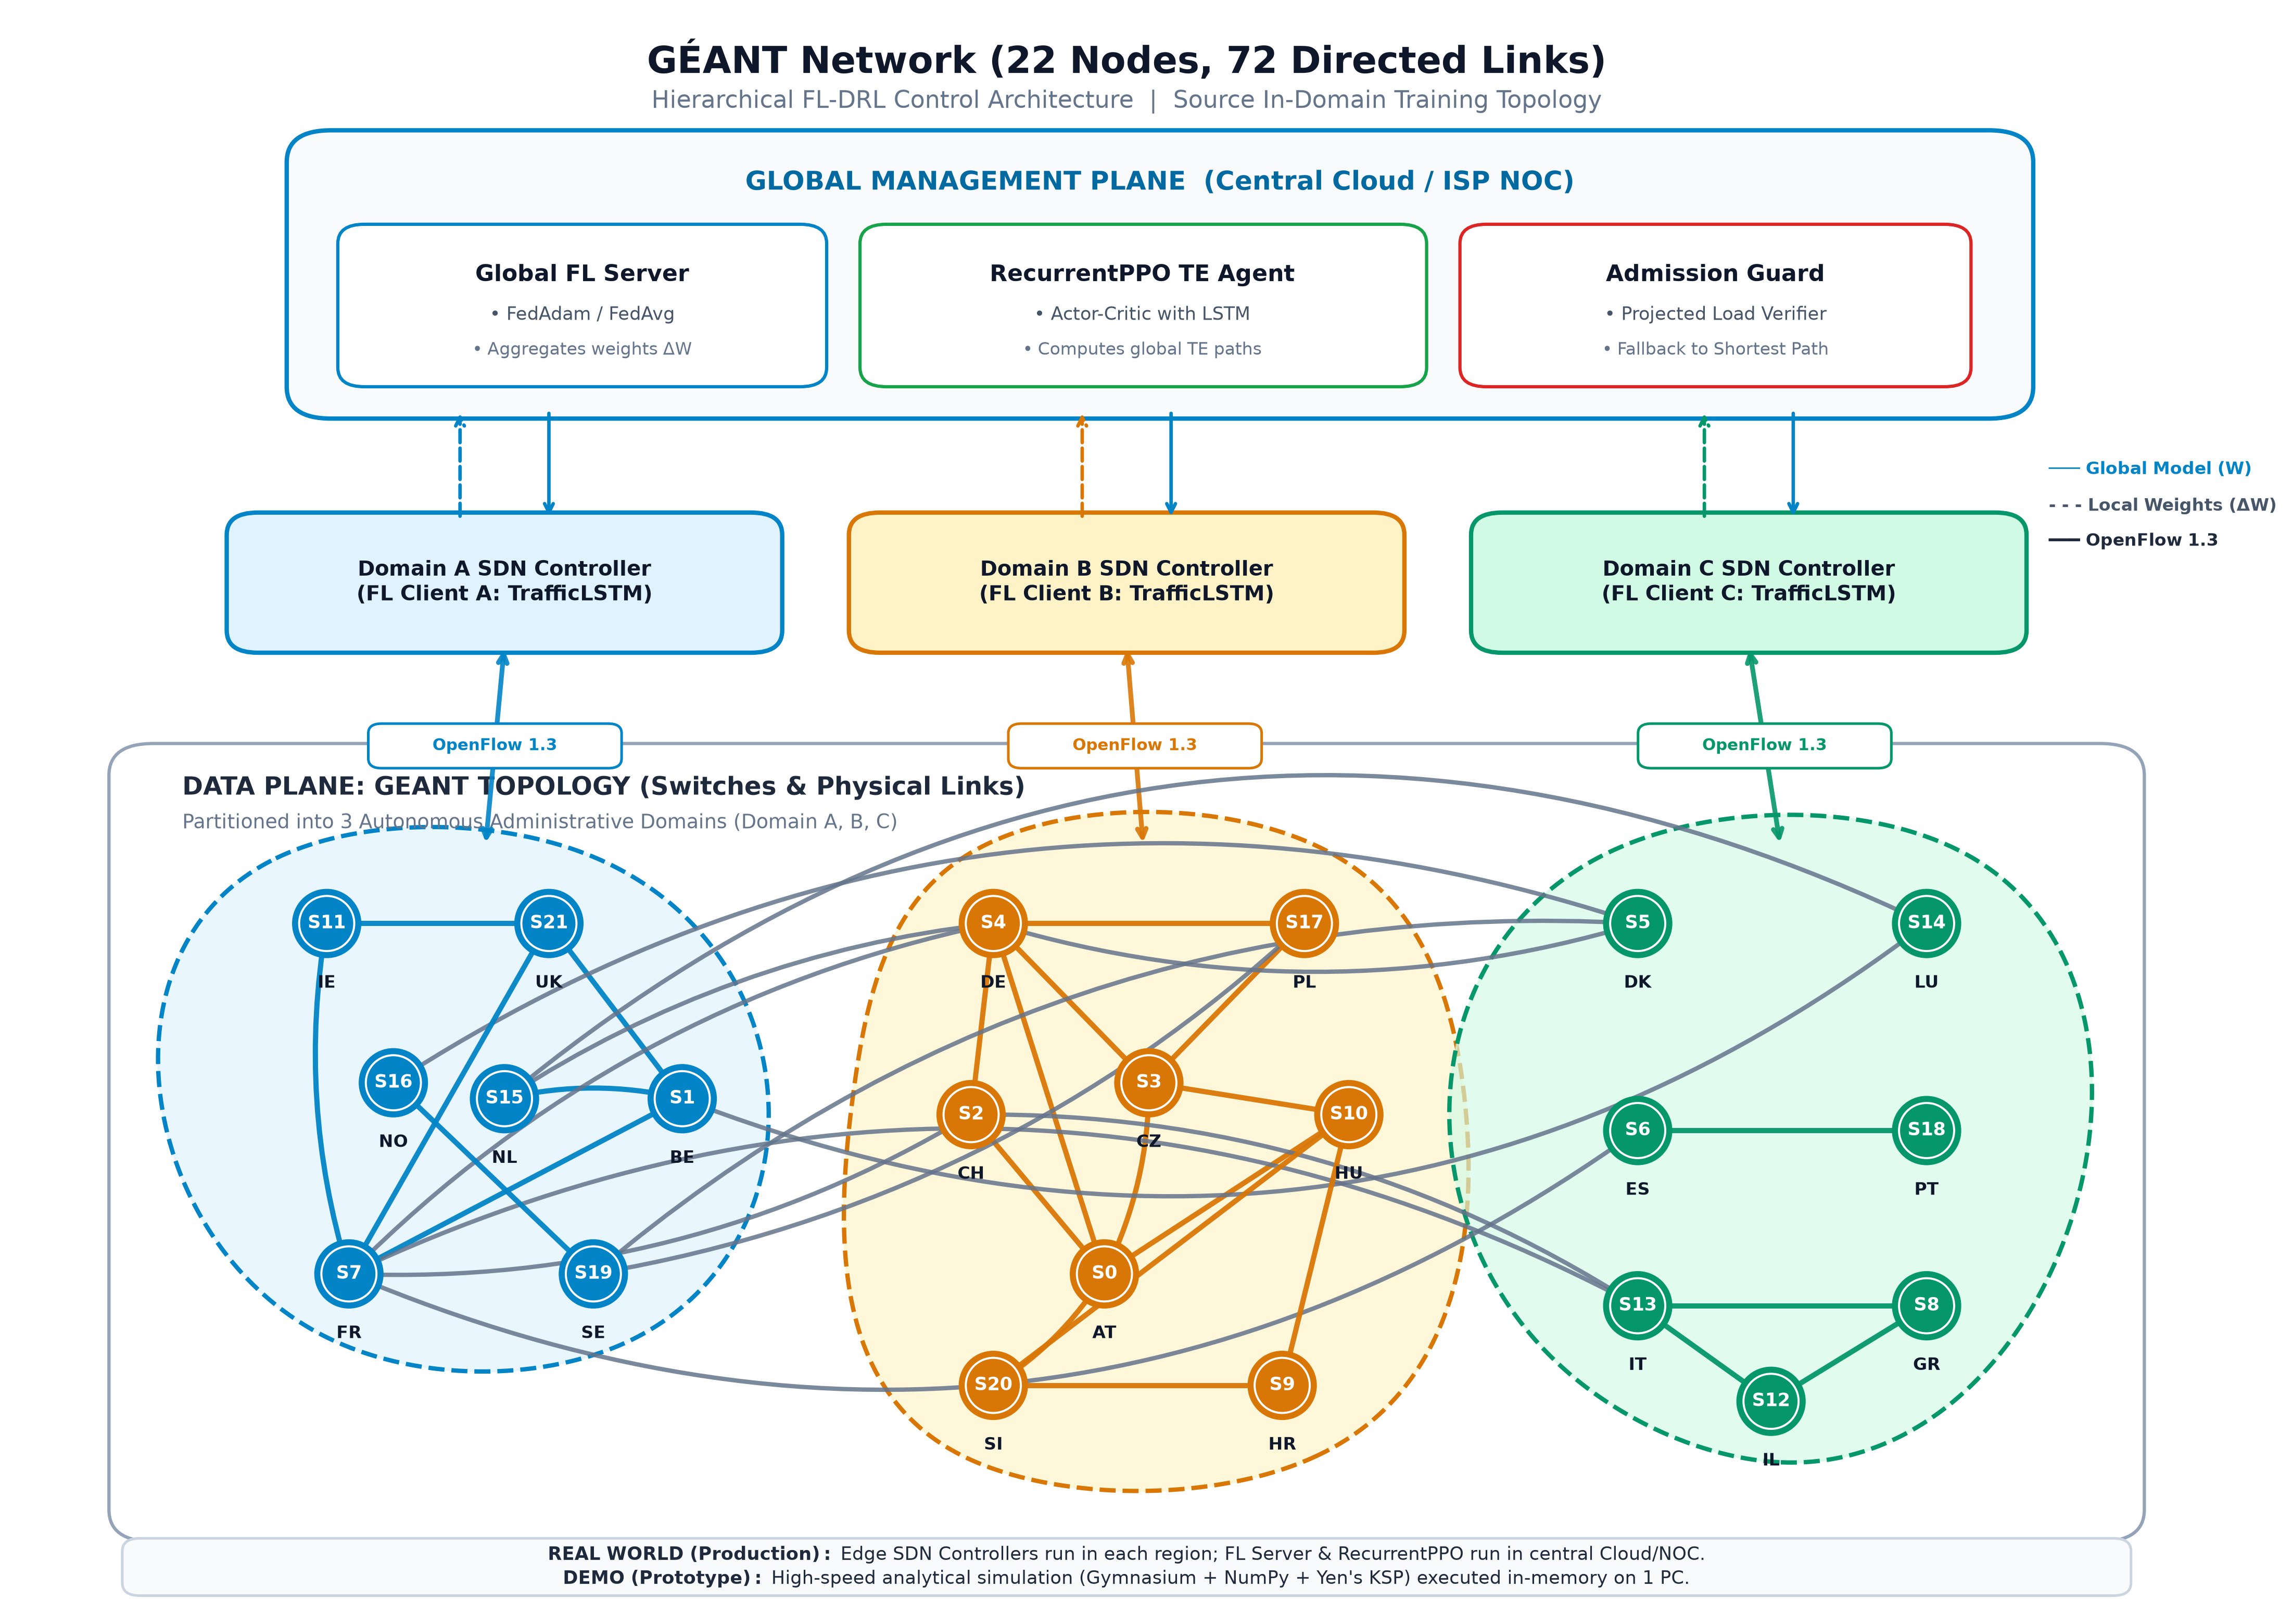
\includegraphics[width=\textwidth]{figures/topology_deployment_geant.png}
        \caption{GÉANT (22 nút, 72 liên kết)}
    \end{subfigure}\hfill
    \begin{subfigure}[b]{0.32\textwidth}
        \centering
        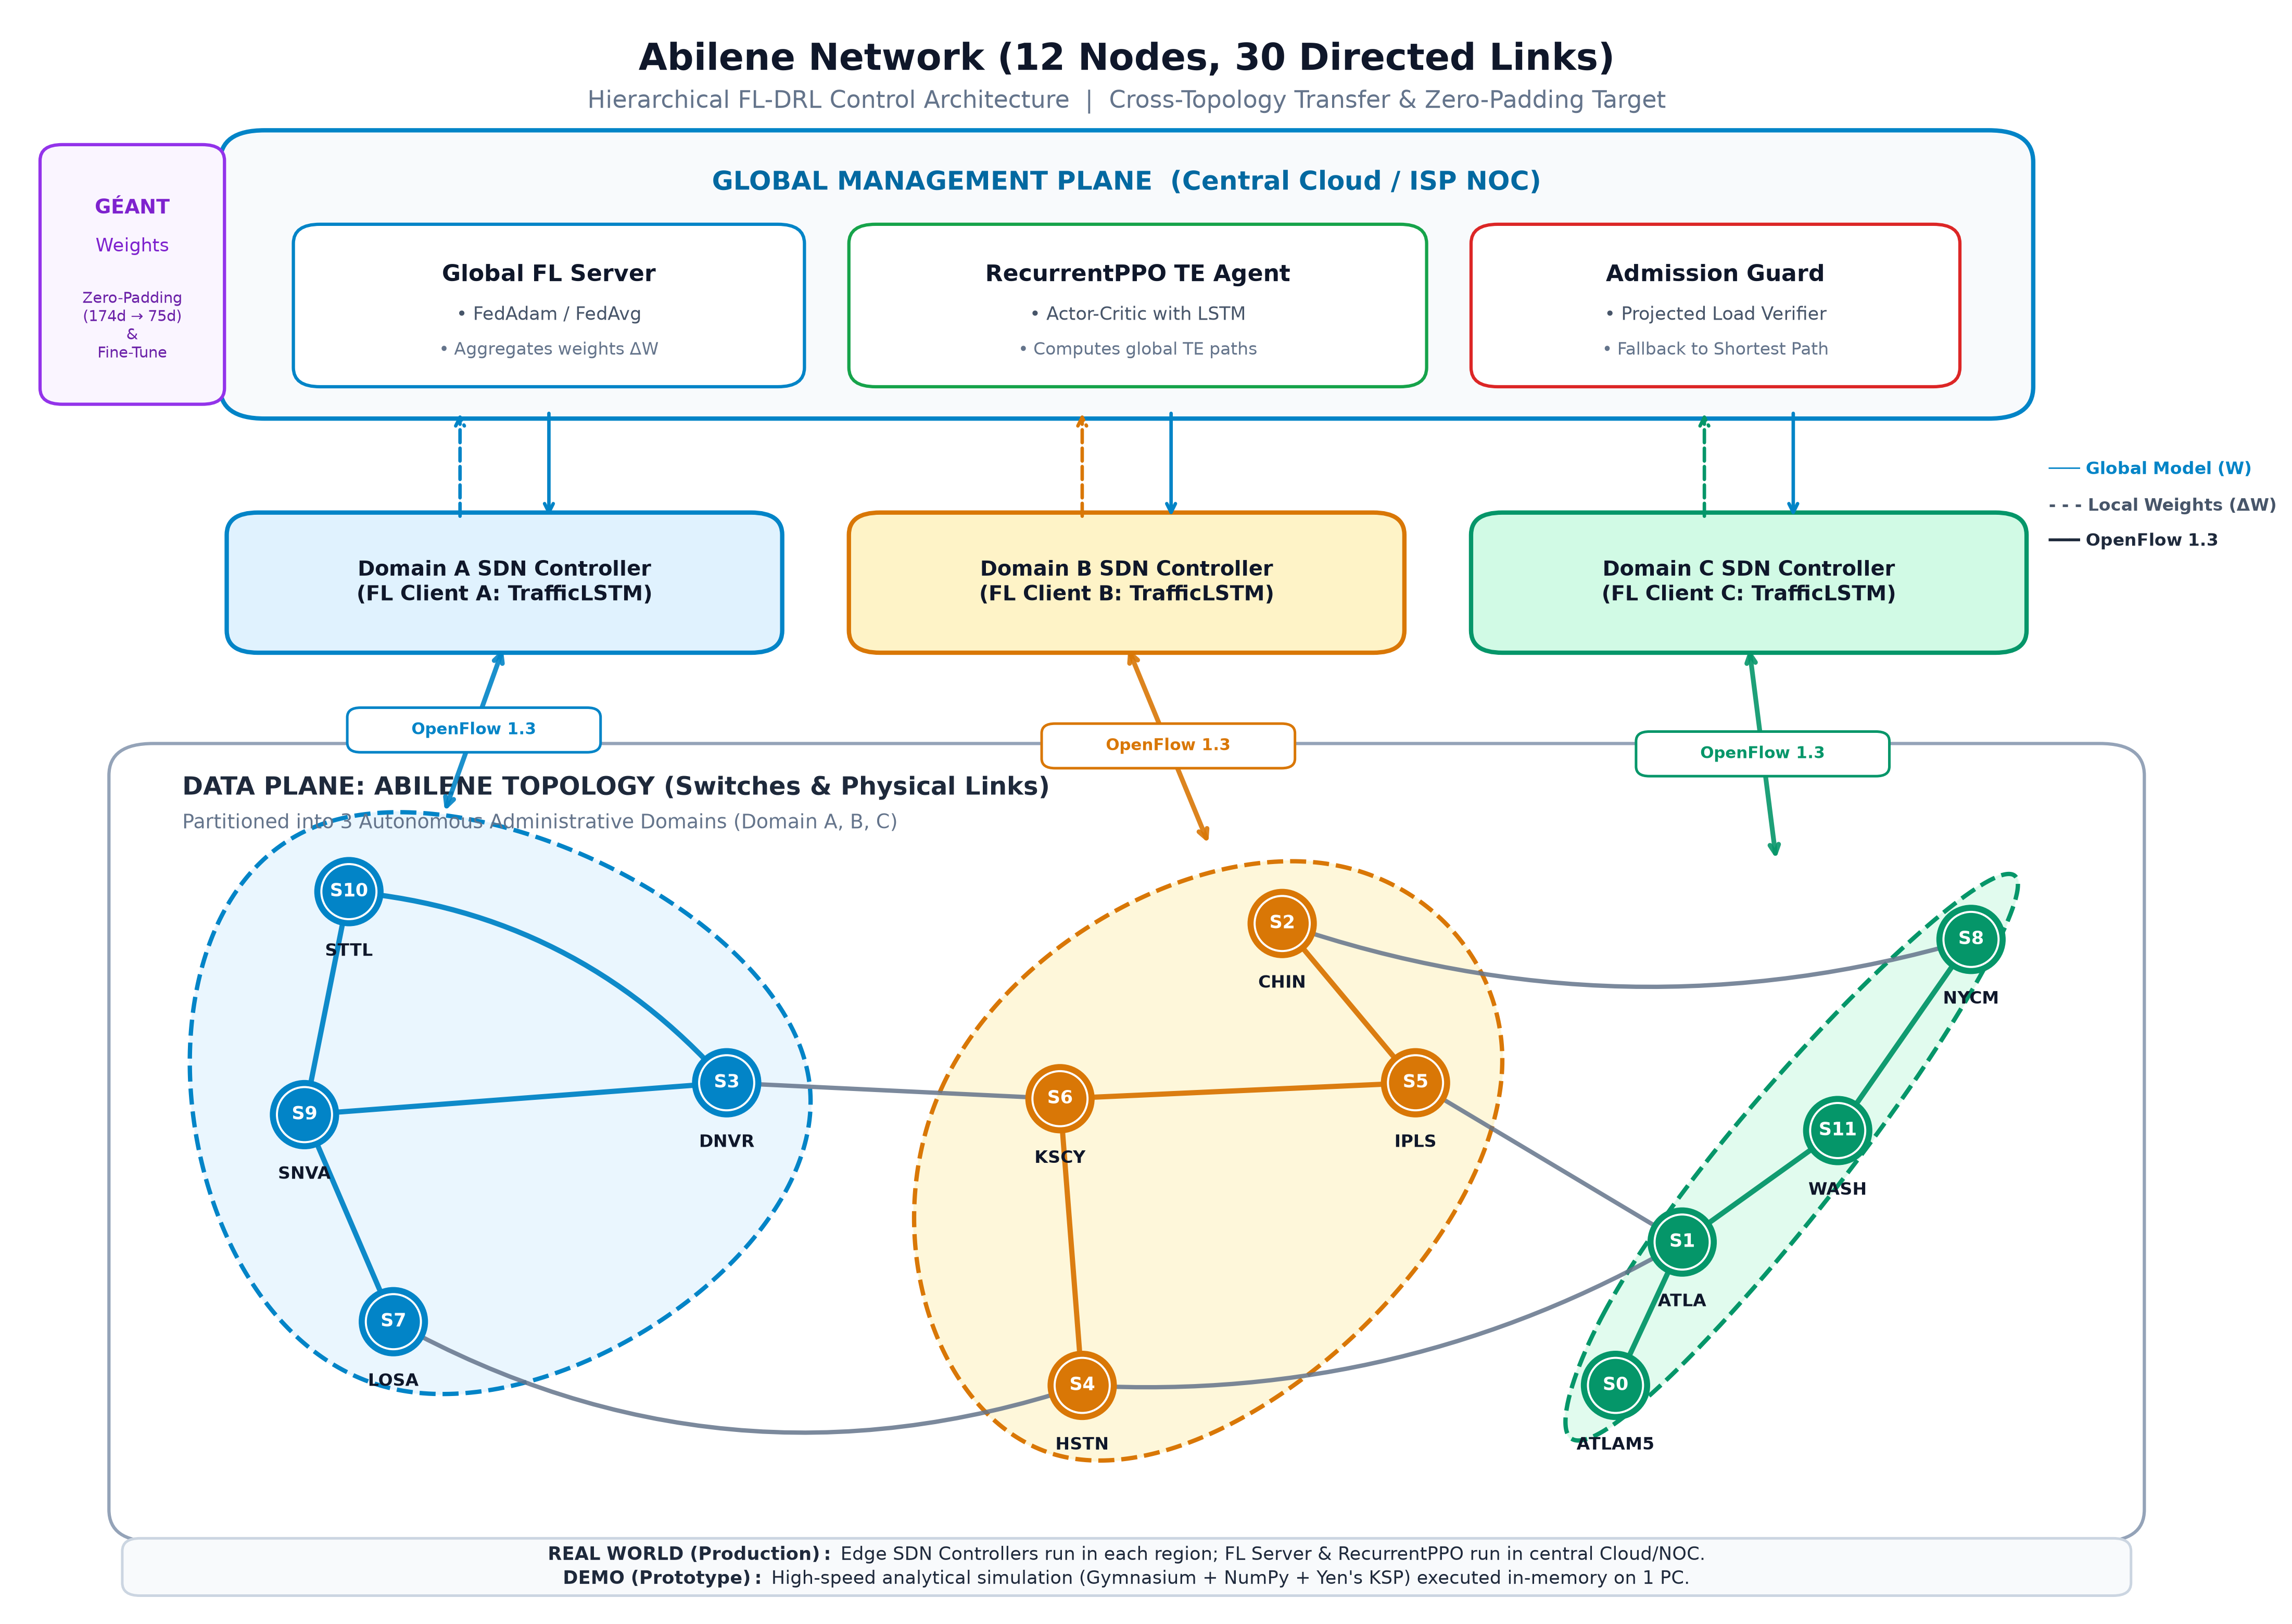
\includegraphics[width=\textwidth]{figures/topology_deployment_abilene.png}
        \caption{Abilene (12 nút, 30 liên kết)}
    \end{subfigure}
    \caption{\textit{Trực quan hóa cấu trúc topo và phân chia 3 miền tự trị (Domain A, B, C) phục vụ huấn luyện FL.}}
    \label{fig:topo_deployments}
\end{figure}

Môi trường huấn luyện Gymnasium (\texttt{rl/env.py}) đã được xây dựng hoàn chỉnh, tích hợp mô hình hàng đợi viễn thông M/M/1 để tính toán chính xác độ trễ lan truyền vật lý, độ trễ xếp hàng dựa trên mức độ chiếm dụng băng thông và xác định tỷ lệ mất gói tức thời khi hàng đợi vượt ngưỡng dung lượng.

\subsection{Xây dựng dữ liệu lưu lượng mạng}
Đã xây dựng chương trình sinh dữ liệu lưu lượng theo Mô hình Hấp dẫn (Gravity Model), mô phỏng chu kỳ ngày/đêm, suy giảm ngày cuối tuần, bùng phát tải cục bộ và sự cố đứt liên kết ngẫu nhiên qua chu kỳ 4 tuần với bước nhảy 15 phút.

Dữ liệu được tiền xử lý và cắt lát theo cửa sổ trượt gồm 12 bước quá khứ ($T=12$, tương đương 3 giờ) để dự đoán 3 bước trong tương lai ($H=3$, tương đương 45 phút nhìn trước) và phân chia theo 3 miền mạng phục vụ huấn luyện FL. Đồng thời, chuỗi ma trận lưu lượng thực nghiệm của GÉANT và Abilene đã được chuẩn hóa để kiểm thử khả năng thích ứng và chuyển giao mô hình.

\subsection{Xây dựng và thiết lập mô hình Federated Learning (TrafficLSTM)}
Đã triển khai kiến trúc học liên kết (Federated Learning) nhằm dự báo chủ động mức độ chiếm dụng của các liên kết mạng diện rộng mà không xâm phạm quyền riêng tư dữ liệu lưu lượng giữa các miền tự trị (Autonomous Systems). Mỗi miền mạng hoạt động như một FL Client độc lập, huấn luyện mô hình dự báo cục bộ trên tập chuỗi thời gian của riêng mình, sau đó chỉ truyền tải sai phân trọng số mô hình về máy chủ trung tâm để tổng hợp thành mô hình toàn cục.

Kiến trúc tổng thể của hệ thống học liên kết đa miền được trực quan hóa tại Hình \ref{fig:fl_architecture}.

\begin{figure}[H]
    \centering
    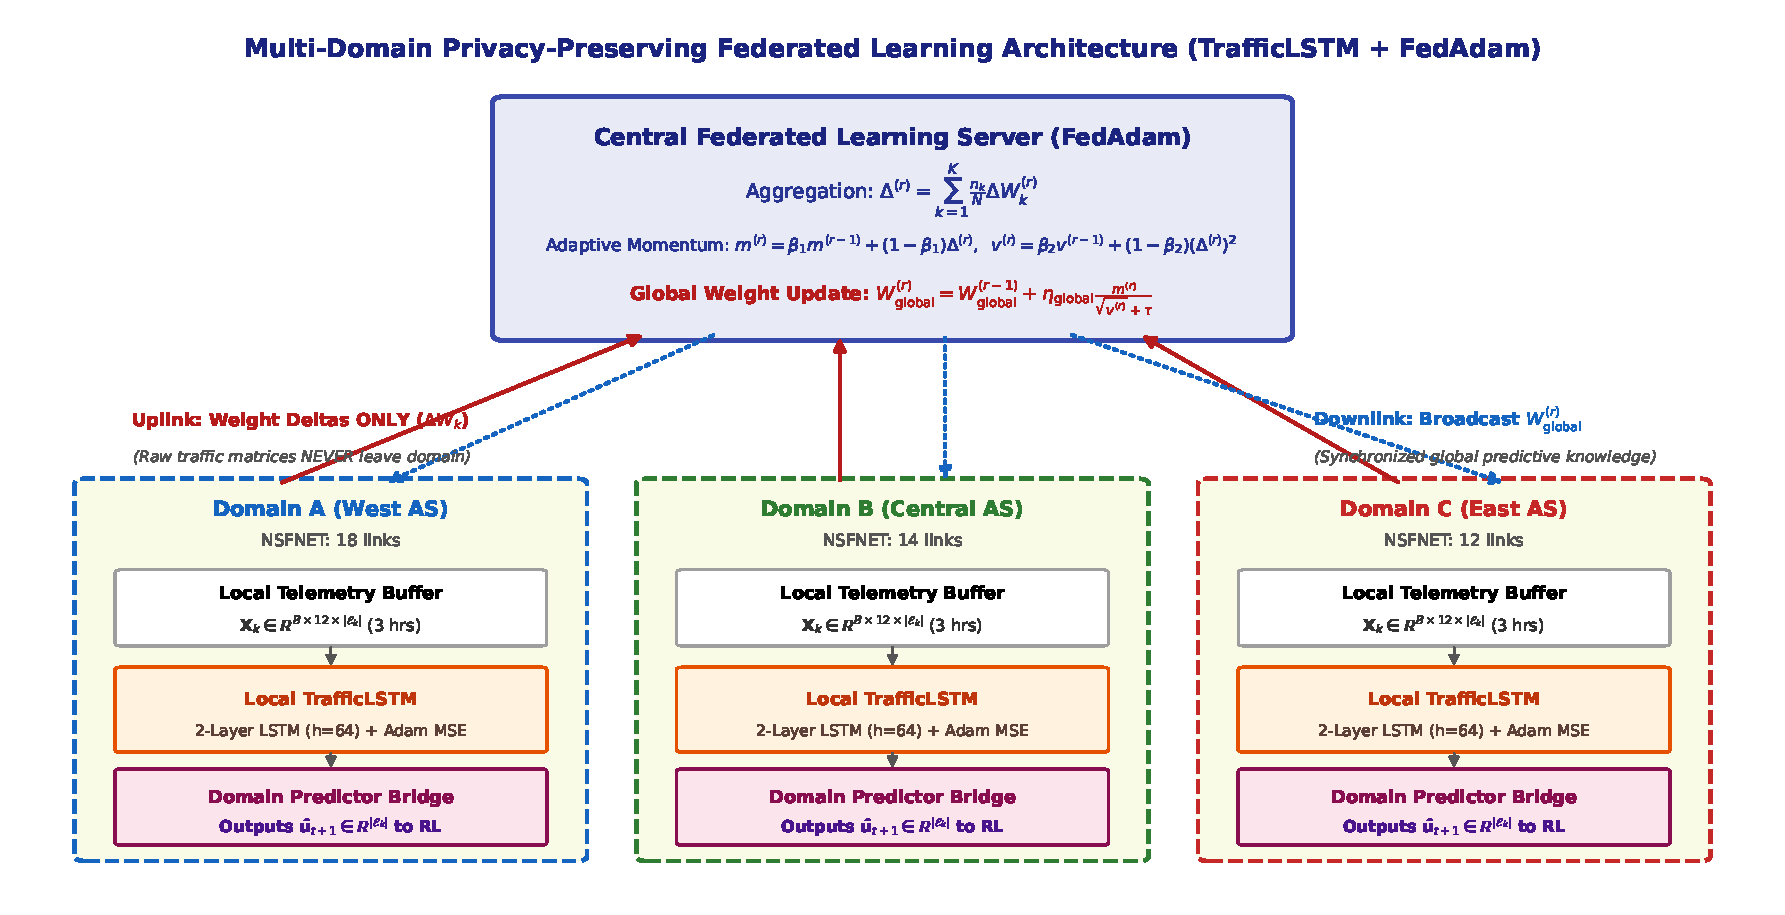
\includegraphics[width=0.96\textwidth]{figures/fig_fl_architecture.pdf}
    \caption{\textit{Kiến trúc học liên kết đa miền bảo toàn quyền riêng tư: Luồng dữ liệu cục bộ, cập nhật sai phân trọng số và thuật toán tổng hợp FedAdam.}}
    \label{fig:fl_architecture}
\end{figure}

Chi tiết dữ liệu đầu vào, đầu ra và cơ chế tối ưu hóa:
\begin{itemize}[leftmargin=1.5em, itemsep=0.2ex]
    \item Dữ liệu đầu vào: Tại mỗi miền mạng $k$, dữ liệu quan sát là mảng 3 chiều $\mathbf{X}_k \in \mathbb{R}^{B \times T \times |\mathcal{E}_k|}$, với kích thước lô $B = 32$, cửa sổ quan sát quá khứ $T = 12$ bước (3 giờ), và $|\mathcal{E}_k|$ là số liên kết có hướng trong miền. Mỗi giá trị là mức chiếm dụng liên kết đã chuẩn hóa: $u_t(e) = \frac{\lambda_t(e)}{C(e)} \in [0.0, 1.0]$.
    \item Đầu ra dự báo: Mô hình dự báo mảng $\mathbf{\hat{Y}}_k \in \mathbb{R}^{B \times H \times |\mathcal{E}_k|}$ với tầm nhìn $H = 3$ bước kế tiếp (45 phút tới), tương ứng với bộ ba vector tải tương lai $[\mathbf{\hat{u}}_{t+1}, \mathbf{\hat{u}}_{t+2}, \mathbf{\hat{u}}_{t+3}]$.
    \item Hàm mất mát tại client: Từng miền $k$ huấn luyện mô hình cục bộ bằng hàm sai số bình phương trung bình (MSE):
    \begin{equation}
        \mathcal{L}_{\text{MSE}}(W_k) = \frac{1}{B \cdot H \cdot |\mathcal{E}_k|} \sum_{b=1}^{B} \sum_{h=1}^{H} \sum_{e \in \mathcal{E}_k} \left( u_{t+h}(e) - \hat{u}_{t+h}(e) \right)^2
    \end{equation}
    \item Cơ chế bảo mật và thuật toán tổng hợp FedAdam: Sau mỗi vòng huấn luyện cục bộ ($E = 5$ epochs), các client chỉ gửi sai phân trọng số $\Delta W_k^{(r)} = W_k^{(r)} - W_{\text{global}}^{(r-1)}$ về máy chủ; dữ liệu lưu lượng nội bộ không bị chia sẻ ra ngoài. Máy chủ FL tổng hợp theo thuật toán \texttt{FedAdam} với động lượng hai bậc để thích ứng với sự khác biệt dữ liệu giữa các miền:
    \begin{align}
        \Delta^{(r)} &= \sum_{k=1}^{K} \frac{n_k}{N} \Delta W_k^{(r)}, \quad m^{(r)} = \beta_1 m^{(r-1)} + (1-\beta_1)\Delta^{(r)} \\
        v^{(r)} &= \beta_2 v^{(r-1)} + (1-\beta_2)(\Delta^{(r)})^2, \quad W_{\text{global}}^{(r)} = W_{\text{global}}^{(r-1)} + \eta_{\text{global}} \frac{m^{(r)}}{\sqrt{v^{(r)}} + \tau}
    \end{align}
    \item Cầu nối sang tác tử RL: Vector tải dự báo ở bước kế tiếp $\mathbf{\hat{u}}_{t+1}$ được trích xuất và nạp thẳng vào trạng thái của tác tử RL: $\mathbf{s}_t = [\mathbf{u}_t \;\parallel\; \mathbf{\hat{u}}_{t+1} \;\parallel\; \mathbf{d}_t]$.
\end{itemize}

\begin{table}[H]
\centering
\caption{\textit{Bảng siêu tham số cấu hình mô hình Federated TrafficLSTM và thuật toán tổng hợp FedAdam.}}
\label{tab:fl_hyperparameters}
\footnotesize
\renewcommand{\arraystretch}{1.02}
\begin{tabularx}{\textwidth}{@{} p{4.6cm} c c X @{}}
\toprule
\textbf{Tham số (Parameter)} & \textbf{Ký hiệu} & \textbf{Giá trị} & \textbf{Mô tả ngắn gọn} \\
\midrule
\multicolumn{4}{@{}l}{\textbf{1. Architecture \& Sequence Parameters (TrafficLSTM)}} \\
Lookback Window & $T$ & 12 steps & 12 bước quan sát quá khứ (3 giờ). \\
Prediction Horizon & $H$ & 3 steps & 3 bước dự báo tương lai (45 phút). \\
LSTM Layers & $L$ & 2 layers & Số tầng LSTM trích xuất đặc trưng chuỗi. \\
Hidden Dimension & $d_{\text{hidden}}$ & 64 units & Kích thước vector trạng thái ẩn. \\
Dropout Rate & $p_{\text{drop}}$ & 0.2 & Tỷ lệ ngắt kết nối chống quá khớp. \\
\midrule
\multicolumn{4}{@{}l}{\textbf{2. Client Training \& FedAdam Optimization}} \\
Mini-batch Size & $B_{\text{FL}}$ & 32 samples & Kích thước lô huấn luyện tại client. \\
Local Epochs & $E$ & 5 epochs & Số lượt huấn luyện cục bộ mỗi vòng. \\
Local Learning Rate & $\eta_{\text{local}}$ & $1 \times 10^{-3}$ & Tốc độ học mô hình cục bộ (Adam, MSE). \\
Global Learning Rate & $\eta_{\text{global}}$ & $1 \times 10^{-3}$ & Tốc độ học tổng hợp toàn cục. \\
FedAdam Momentum & $\beta_1, \beta_2$ & 0.9, 0.99 & Hệ số động lượng thuật toán FedAdam. \\
Global Communication Rounds & $R$ & 50 rounds & Số vòng tổng hợp tham số toàn cục. \\
\bottomrule
\end{tabularx}
\end{table}

\subsection{Xây dựng và thiết lập môi trường Reinforcement Learning (RecurrentPPO)}
Môi trường Gymnasium (\texttt{rl/env.py}) phục vụ huấn luyện tác tử điều khiển lưu lượng theo cơ chế vòng lặp kín (Closed-Loop Routing). Thiết lập kỹ thuật gồm các điểm chính:

\begin{itemize}[leftmargin=1.5em, itemsep=0.3ex]
    \item Không gian trạng thái: Vector quan sát tại mỗi bước thời gian $t$ ghép nối 3 thành phần thông tin:
    \begin{equation}
        \mathbf{s}_t = \left[ \mathbf{u}_t \;\parallel\; \mathbf{\hat{u}}_{t+1} \;\parallel\; \mathbf{d}_t \right] \in \mathbb{R}^{2|\mathcal{E}| + |\mathcal{M}|}
    \end{equation}
    trong đó $\mathbf{u}_t$ là mức tải hiện tại của các liên kết, $\mathbf{d}_t$ là nhu cầu lưu lượng của các luồng lớn quản lý, và $\mathbf{\hat{u}}_{t+1}$ là mức tải dự báo ở bước kế tiếp từ mô hình Federated TrafficLSTM. Nhờ vector dự báo này, tác tử có thể nhận biết sớm nguy cơ nghẽn để chủ động đổi hướng luồng trước khi hàng đợi gói tin bị đầy.
    
    \item Không gian hành động đa rời rạc (MultiDiscrete): Thay vì điều khiển toàn bộ ma trận lưu lượng, hệ thống chỉ tập trung kiểm soát nhóm luồng lớn (chiếm hơn 85\% tổng tải): 20 luồng trên NSFNET, 30 luồng trên GÉANT và 15 luồng trên Abilene. Với mỗi luồng lớn, thuật toán Yen tìm sẵn $K = 3$ đường đi ngắn nhất. Tác tử chọn 1 trong 3 đường cho từng luồng lớn, còn các luồng nhỏ còn lại mặc định chạy trên đường ngắn nhất OSPF.
\end{itemize}

\subsubsection*{Lý do lựa chọn thuật toán PPO và tầng nhớ LSTM}
Việc lựa chọn RecurrentPPO (PPO kết hợp LSTM) thay vì các thuật toán RL khác (như DQN) hay mạng MLP thông thường dựa trên các lý do chính sau:

\begin{enumerate}[leftmargin=1.5em, itemsep=0.3ex]
    \item Tránh bùng nổ không gian hành động: Với 20--30 luồng lớn và mỗi luồng có 3 lựa chọn đường đi, nếu gộp chung thành một không gian rời rạc đơn lẻ như trong DQN, số hành động kết hợp sẽ lên tới $3^{20} \approx 3.48 \times 10^9$ (NSFNET) hoặc $3^{30} \approx 2.05 \times 10^{14}$ (GÉANT). Không gian này quá lớn để DQN có thể học được. PPO hỗ trợ không gian \texttt{MultiDiscrete}, cho phép tác tử chọn đường cho từng luồng một cách độc lập:
    \begin{equation}
        \pi_\theta(\mathbf{a}_t \mid \mathbf{s}_t) = \prod_{k \in \mathcal{M}} \pi_{\theta_k}(a_t[k] \mid \mathbf{s}_t)
    \end{equation}
    Nhờ đó, mạng chính sách chỉ cần xuất ra $3 \times 20 = 60$ giá trị đầu ra (tăng tuyến tính theo số luồng), giúp mô hình học nhanh và ổn định hơn rất nhiều.
    
    \item Cập nhật chính sách an toàn với cơ chế PPO Clip: Lưu lượng mạng viễn thông biến động rất nhanh và độ trễ tăng vọt khi nghẽn. Các thuật toán Policy Gradient thông thường rất dễ bị hỏng chính sách nếu cập nhật bước nhảy quá lớn khi gặp đột biến tải. PPO giải quyết vấn đề này bằng hàm mục tiêu cắt tỉa:
    \begin{equation}
        \mathcal{L}^{\text{CLIP}}(\theta) = \hat{\mathbb{E}}_t \left[ \min\left( r_t(\theta)\hat{A}_t, \, \text{clip}(r_t(\theta), 1-\epsilon_{\text{clip}}, 1+\epsilon_{\text{clip}})\hat{A}_t \right) \right]
    \end{equation}
    với $\epsilon_{\text{clip}} = 0.2$. Cơ chế này giới hạn mức thay đổi chính sách ở mỗi bước cập nhật, giúp quá trình học diễn ra êm và không bị sụp đổ khi gặp biến động bất thường.
    
    \item Tầng nhớ LSTM giúp nhận biết xu hướng lưu lượng: Một trạng thái $\mathbf{s}_t$ tại thời điểm hiện tại chỉ là ảnh chụp tĩnh, không cho biết tải đang tăng, đang giảm hay đi ngang. Tầng nhớ LSTM (128 đơn vị) lưu lại ngữ cảnh chuỗi thời gian của các bước trước đó, giúp tác tử nắm bắt được xu hướng biến thiên của lưu lượng mạng.
    
    \item Tránh rung giật tuyến (Route Flapping): Mạng truyền thẳng (MLP) thông thường rất dễ bị hiện tượng đổi đường liên tục ở mỗi bước thời gian khi tải dao động quanh ngưỡng $0.65$. Hiện tượng nhảy tuyến này làm đảo lộn thứ tự gói tin TCP và làm giảm thông lượng mạng. Nhờ bộ nhớ trạng thái ẩn, LSTM tạo ra quán tính hành động (Action Inertia): tác tử sẽ giữ nguyên tuyến đường ổn định khi tải chỉ dao động nhẹ (tỷ lệ đổi tuyến $\text{Churn} < 0.1\%$), và chỉ chuyển hướng khi tải tăng cao rõ rệt hoặc khi có sự cố đứt đường truyền.
\end{enumerate}

\begin{figure}[H]
    \centering
    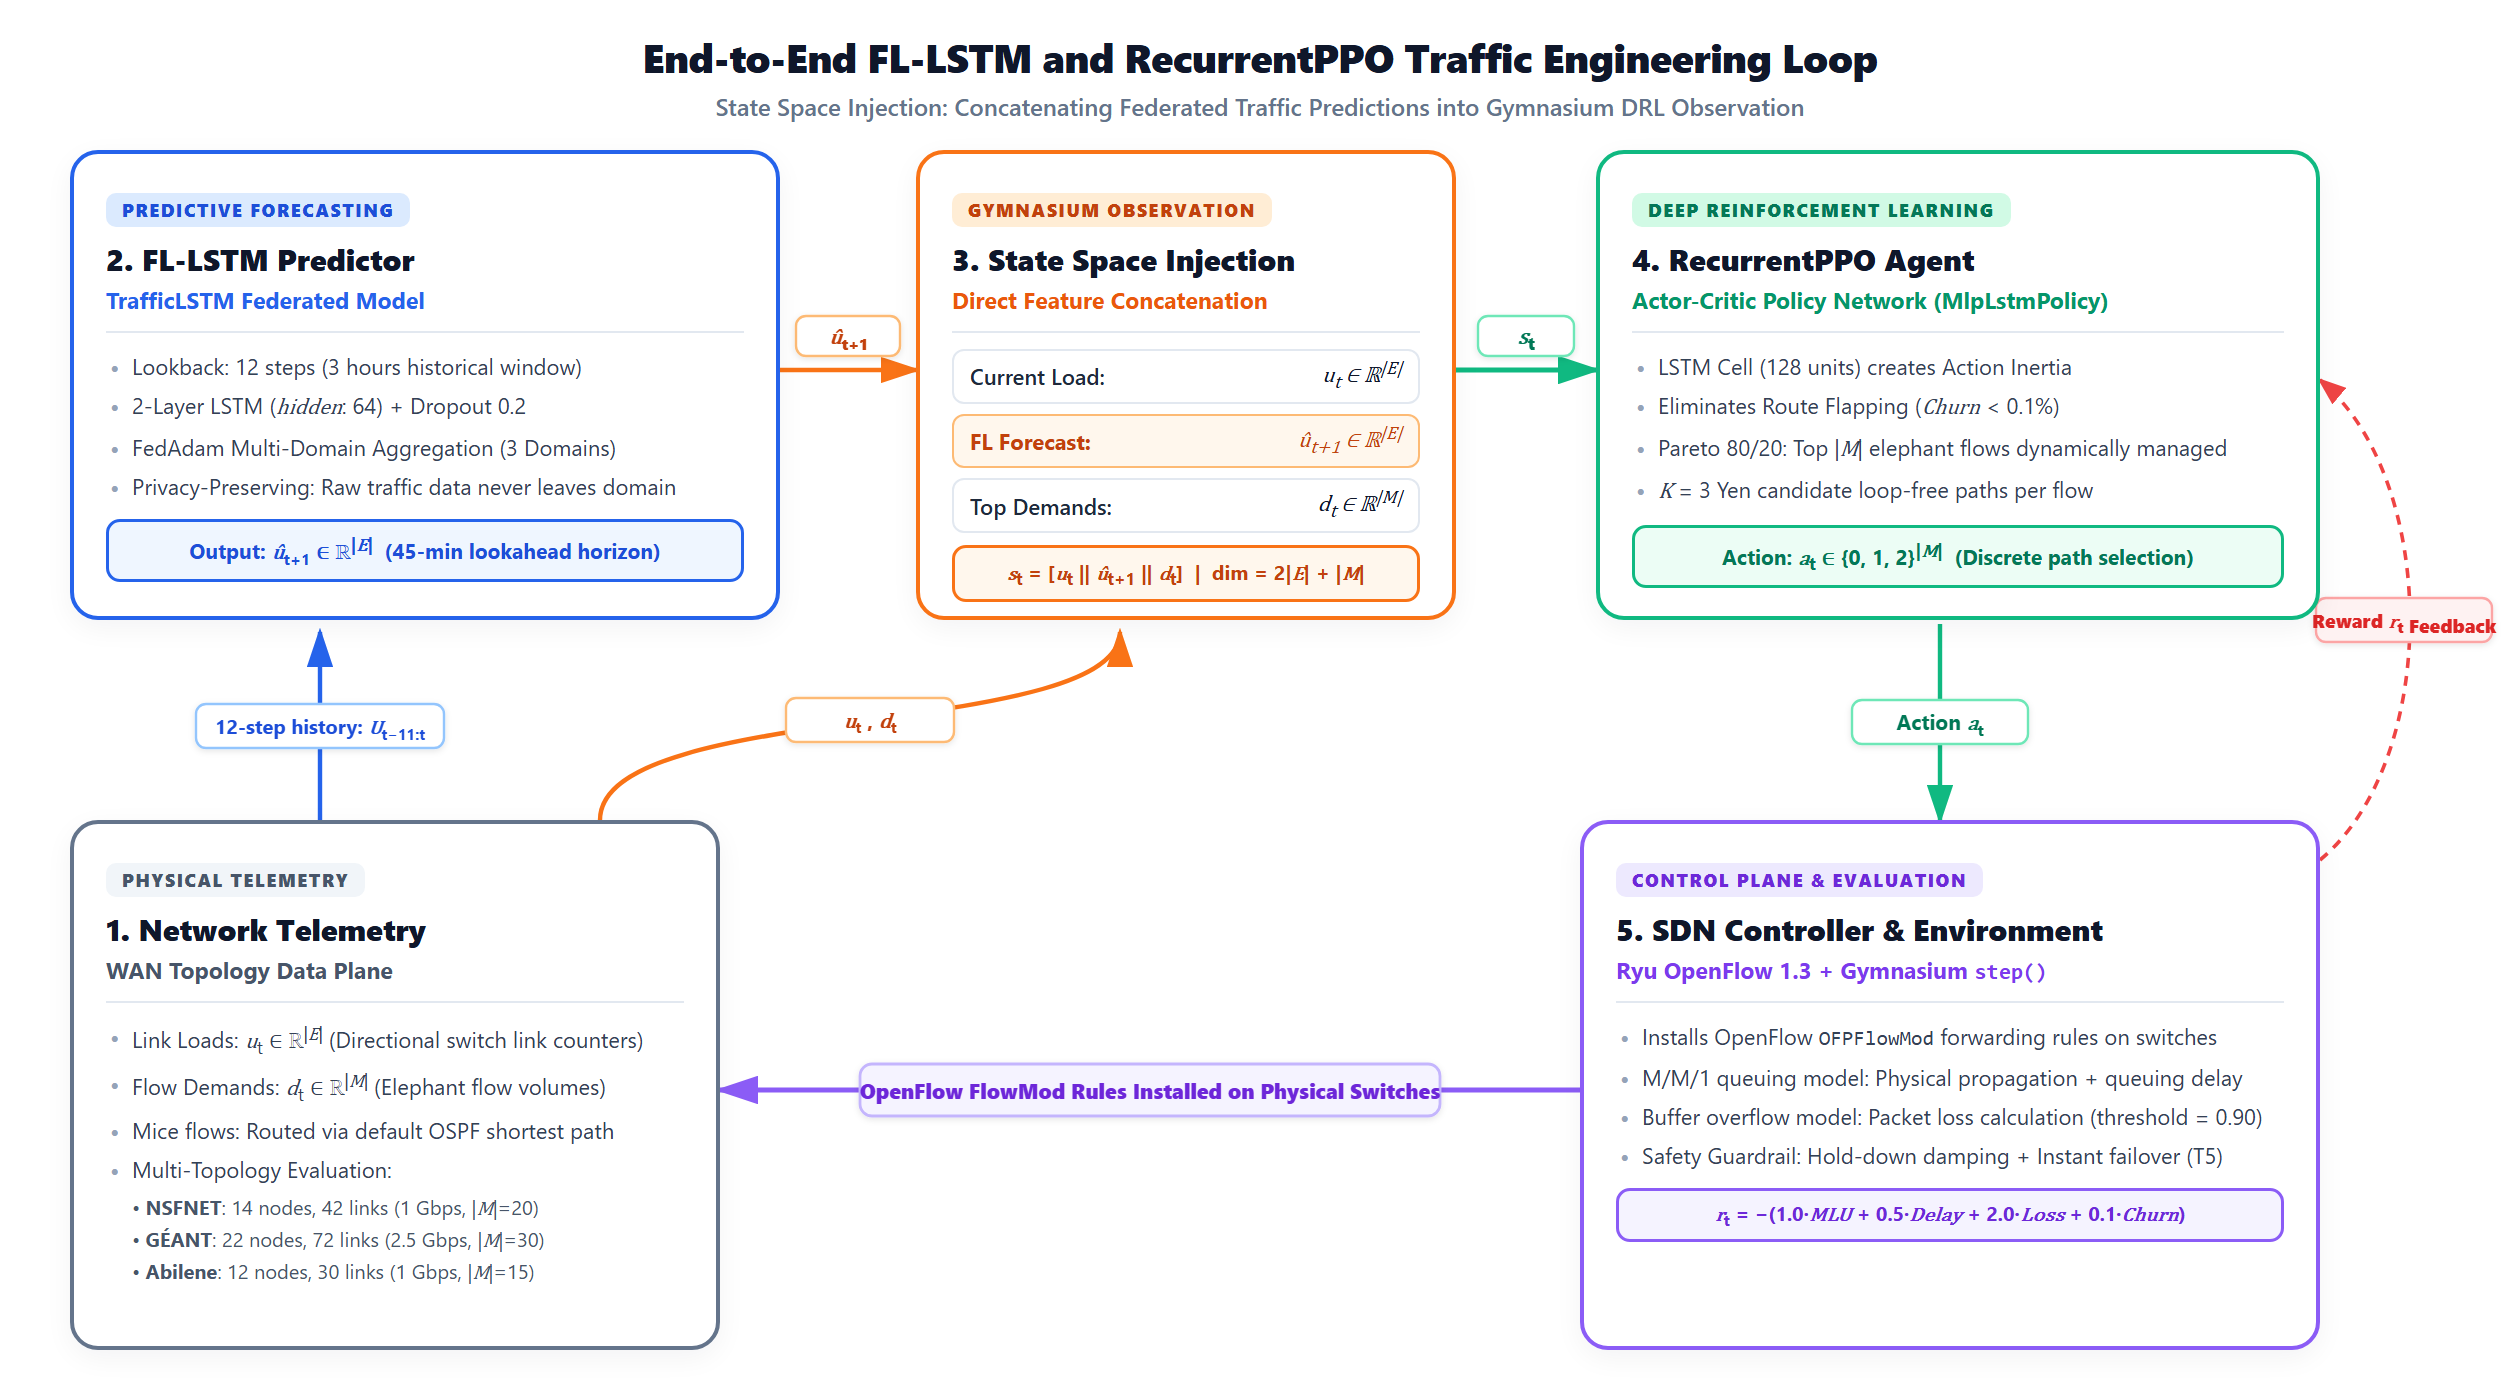
\includegraphics[width=0.96\textwidth]{figures/fig_lstm_ppo_env.png}
    \caption{\textit{Sơ đồ vòng lặp điều khiển lưu lượng giữa FL-LSTM, RecurrentPPO và SDN.}}
    \label{fig:lstm_ppo_env}
\end{figure}

\begin{table}[H]
\centering
\caption{\textit{Bảng cấu hình siêu tham số mô hình định tuyến \texttt{RecurrentPPO}.}}
\label{tab:rl_hyperparameters}
\footnotesize
\renewcommand{\arraystretch}{1.02}
\begin{tabularx}{\textwidth}{@{} p{4.6cm} c c X @{}}
\toprule
\textbf{Tham số (Parameter)} & \textbf{Ký hiệu} & \textbf{Giá trị} & \textbf{Mô tả ngắn gọn} \\
\midrule
\multicolumn{4}{@{}l}{\textbf{1. Policy Network Architecture (MlpLstmPolicy)}} \\
Policy Class & -- & \texttt{MlpLstm} & Mạng Actor-Critic có bộ nhớ ẩn LSTM. \\
LSTM Hidden Units & $d_{\text{lstm}}$ & 128 units & Kích thước vector trạng thái ẩn LSTM. \\
Actor Network ($\pi_\theta$) & MLP & $[256, 128]$ & Đầu ra xác suất chọn tuyến ($K=3$). \\
Critic Network ($V_\phi$) & MLP & $[256, 128]$ & Đầu ra ước lượng giá trị trạng thái $V(\mathbf{s}_t)$. \\
\midrule
\multicolumn{4}{@{}l}{\textbf{2. RecurrentPPO Optimization \& GAE}} \\
Rollout Buffer & $N_{\text{steps}}$ & 1024 steps & Bộ đệm rollout (8 môi trường song song $\times$ 128 bước). \\
Mini-batch Size & $B_{\text{RL}}$ & 64 samples & Kích thước mẫu cập nhật gradient. \\
Update Epochs & $K_{\text{epoch}}$ & 10 epochs & Số lượt tối ưu chính sách mỗi đợt rollout. \\
Learning Rate Schedule & $\alpha$ & $3 \cdot 10^{-4} \to 1 \cdot 10^{-4}$ & Suy giảm tuyến tính theo tiến trình học. \\
Discount Factor & $\gamma$ & 0.95 & Hệ số chiết khấu phần thưởng tương lai. \\
GAE Coefficient & $\lambda_{\text{GAE}}$ & 0.95 & Hệ số ước lượng lợi thế (GAE). \\
PPO Clip Range & $\epsilon_{\text{clip}}$ & 0.2 & Ngưỡng cắt tỉ số xác suất chính sách. \\
Value Loss Coefficient & $c_1$ & 0.5 & Trọng số mất mát của Critic trong tổng hàm loss. \\
Entropy Coefficient & $c_2$ & 0.001 & Trọng số entropy khuyến khích khám phá. \\
Max Gradient Norm & $g_{\text{max}}$ & 0.5 & Ngưỡng cắt chuẩn gradient chống bùng nổ. \\
\bottomrule
\end{tabularx}
\end{table}

\subsection{Xây dựng hàm đánh giá môi trường và phân tích hàm phần thưởng}
Hàm \texttt{step()} trong môi trường Gymnasium mô phỏng phản ứng của mạng sau mỗi quyết định định tuyến: gán đường đi cho các luồng, cộng dồn lưu lượng lên từng liên kết, tính mức tải cực đại (MLU), tính độ trễ lan truyền và độ trễ hàng đợi theo mô hình M/M/1, kiểm tra tỷ lệ mất gói và tính điểm phần thưởng.

Quy trình thực thi logic chuyển trạng thái của môi trường được mô tả tại Thuật toán \ref{alg:gym_step}:

\begin{algorithm}[H]
\caption{Quy trình một bước chuyển trạng thái (Gym Environment Step)}
\label{alg:gym_step}
\begin{algorithmic}[1]
\Require Vector hành động $\text{actions}$, ma trận lưu lượng $\text{traffic\_matrix}$.
\Ensure Trạng thái mới $s_{t+1}$, phần thưởng $R_t$, cờ kết thúc $done$, thông tin chẩn đoán $info$.

\State 1. Chọn đường đi cho các luồng lớn từ tập K đường ngắn nhất:
\State \quad \texttt{for flow in managed\_flows:}
\State \quad \quad \texttt{path[flow] = K\_shortest\_paths[flow][actions[flow]]}

\State 2. Định tuyến các luồng nhỏ còn lại qua đường ngắn nhất OSPF:
\State \quad \texttt{for flow in background\_flows:}
\State \quad \quad \texttt{path[flow] = ospf\_shortest\_path(flow)}

\State 3. Cộng dồn lưu lượng lên từng liên kết mạng:
\State \quad \texttt{for link in links:}
\State \quad \quad \texttt{link\_load[link] = sum(flow.demand for flow in flows\_using\_link)}

\State 4. Tính mức sử dụng liên kết và tải cực đại toàn mạng (MLU):
\State \quad \texttt{for link in links:}
\State \quad \quad \texttt{util[link] = link\_load[link] / link\_capacity[link]}
\State \quad \texttt{MLU = max(util.values())}

\State 5. Tính độ trễ lan truyền và trễ hàng đợi M/M/1:
\State \quad \texttt{for link in links:}
\State \quad \quad \texttt{delay[link] = prop\_delay[link] + mm1\_queue\_delay(util[link])}

\State 6. Đánh giá tỷ lệ mất gói khi tải vượt ngưỡng 90\%:
\State \quad \texttt{for link in links:}
\State \quad \quad \texttt{loss[link] = ((util[link] - 0.9) / 0.1)**2 if util[link] > 0.9 else 0.0}

\State 7. Đo đạc tỷ lệ nhảy tuyến (Route Churn) so với bước trước:
\State \quad \texttt{flapped = count(actions[flow] != prev\_actions[flow])}
\State \quad \texttt{churn = flapped / total\_managed\_flows}

\State 8. Điều chỉnh trọng số phạt trễ theo mức tải mạng:
\State \quad \texttt{w\_delay = 0.8 if MLU < 0.65 else 0.3}

\State 9. Tính điểm phần thưởng tổng hợp:
\State \quad \texttt{penalty = 1.0 * MLU + 0.5 * norm\_delay + w\_delay * excess\_delay}
\State \quad \texttt{reward = -(penalty + 3.0 * loss + 0.08 * churn)}

\State 10. Lấy dự báo tải từ mô hình FL và ghép vector trạng thái mới:
\State \quad \texttt{predicted\_load = federated\_lstm.predict(recent\_load\_history)}
\State \quad \texttt{next\_state = concatenate([current\_util, predicted\_load, current\_demands])}

\State \Return \texttt{next\_state, reward, done, info}
\end{algorithmic}
\end{algorithm}

Hàm phần thưởng được thiết kế nhằm cân bằng giữa việc giảm nghẽn mạng và duy trì độ trễ thấp:
\begin{equation}
\label{eq:reward}
    R_t = -\left( 1.0 \cdot \text{MLU}_t + 0.5 \cdot \bar{D}_t^{\text{norm}} + w_{\text{delay}}(t) \cdot D_t^{\text{excess}} + 3.0 \cdot \bar{L}_t + 0.08 \cdot \text{Churn}_t \right)
\end{equation}

Ý nghĩa và cơ sở lựa chọn các trọng số trong hàm phần thưởng:
\begin{itemize}[leftmargin=1.5em, itemsep=0.15ex]
    \item Trễ chuẩn hóa ($0.5 \cdot \bar{D}_t^{\text{norm}}$): Đưa độ trễ trung bình $\bar{D}_t$ về miền $[0, 1]$ cùng thang đo với MLU để giữ độ ổn định gradient và duy trì áp lực giảm trễ.
    \item Trễ đường vòng ($D_t^{\text{excess}}$): Đo tỷ lệ độ trễ tăng thêm khi chọn đường phụ so với đường ngắn nhất OSPF ($D_{\text{base}}$).
    \item Phạt trễ khi tải thấp ($w_{\text{delay}} = 0.8$ khi $\text{MLU} < 0.65$): Phạt nặng việc đi đường vòng để ép các luồng chạy trên đường ngắn nhất OSPF khi mạng đang thông thoáng.
    \item Phạt trễ khi tải cao ($w_{\text{delay}} = 0.3$ khi $\text{MLU} \ge 0.65$): Giảm phạt đường vòng để tác tử được phép rẽ luồng sang đường phụ nhằm giảm tải và tránh nghẽn.
    \item Phạt mất gói ($3.0 \cdot \bar{L}_t$): Trọng số phạt cao để ngăn chặn việc đánh đổi làm rơi gói tin lấy độ trễ thấp.
    \item Phạt nhảy tuyến ($0.08 \cdot \text{Churn}_t$): Hạn chế việc đổi tuyến liên tục giữa các bước, giúp luồng truyền TCP ổn định hơn.
\end{itemize}

\begin{figure}[H]
    \centering
    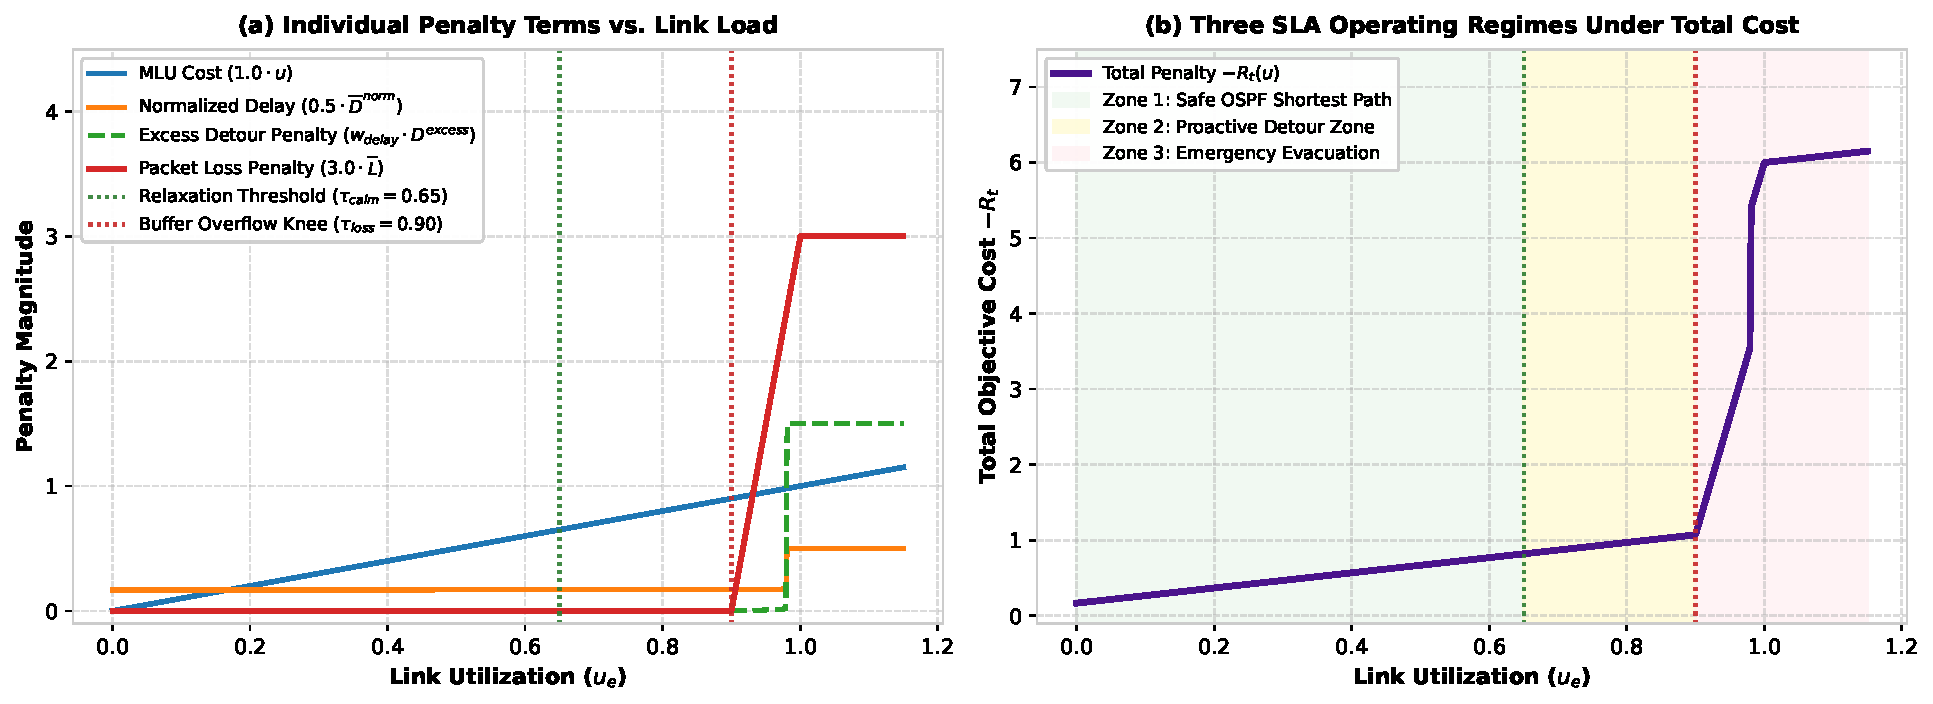
\includegraphics[width=0.96\textwidth]{figures/fig_reward_proof.pdf}
    \caption{\textit{Phân tích đồ thị hàm phần thưởng: (a) Mức phạt của từng thành phần theo mức tải liên kết $u$; (b) Phân vùng 3 trạng thái hoạt động (Safe Zone, Proactive Detour Zone, Emergency Evacuation Zone).}}
    \label{fig:reward_proof}
\end{figure}

\subsubsection*{Phân tích 3 vùng vận hành của hàm phần thưởng}
Đồ thị Hình \ref{fig:reward_proof} minh họa cách hàm phần thưởng tự động phân hóa hành vi định tuyến thành 3 vùng theo mức tải liên kết $u$:

\begin{enumerate}[leftmargin=1.5em, itemsep=0.3ex]
    \item Vùng an toàn ($u < 0.65$): Khi tải mạng thấp, hàng đợi M/M/1 xấp xỉ 0 và không có mất gói. Lúc này, đi đường vòng chỉ làm tăng trễ lan truyền. Do trọng số phạt trễ đường vòng ở mức cao ($w_{\text{delay}} = 0.8$), mô hình sẽ luôn giữ luồng trên đường ngắn nhất OSPF.
    
    \item Vùng rẽ nhánh chủ động ($0.65 \le u \le 0.90$): Khi tải vượt 0.65, trễ hàng đợi bắt đầu tăng nhanh. Hệ thống tự động giảm phạt trễ đường vòng xuống $w_{\text{delay}} = 0.3$. Lúc này, chi phí phạt tải cao ($1.0 \times \text{MLU}$) lớn hơn chi phí đi đường vòng ($0.3 \times D^{\text{excess}}$), thúc đẩy tác tử chủ động chuyển bớt luồng lớn sang đường phụ để san tải và tránh nghẽn trước khi bộ đệm bị tràn.
    
    \item Vùng di tản khẩn cấp ($u > 0.90$): Khi tải vượt ngưỡng 0.90, hàng đợi bị tràn và gói tin bắt đầu rơi. Thành phần phạt mất gói với trọng số 3.0 tăng vọt và chiếm ưu thế áp đảo toàn bộ các thành phần khác (Hình \ref{fig:reward_proof}a). Tác tử buộc phải chuyển luồng ra khỏi liên kết nghẽn ngay lập tức để cứu gói tin, chấp nhận đi đường vòng xa hơn hoặc đổi tuyến tạm thời.
\end{enumerate}

\subsection{Đặc tả chi tiết các kịch bản đánh giá}
Hệ thống sử dụng bộ 6 kịch bản thực nghiệm trên chu kỳ 100 bước ($\Delta t = 15$ phút/bước, tương đương 25 giờ). Gọi $\mathbf{TM}_t(u, v)$ là nhu cầu lưu lượng giữa cặp nút $(u, v)$ tại bước $t$, và $\mathbf{TM}^{\text{base}}(u, v)$ là ma trận lưu lượng danh định cơ sở:

\begin{itemize}[leftmargin=1.5em, itemsep=0.3ex]
    \item T1 (Chu kỳ ngày/đêm): Lưu lượng biến thiên hình sin theo chu kỳ 24 giờ tự nhiên:
    \begin{equation}
        \mathbf{TM}_t(u, v) = \mathbf{TM}^{\text{base}}(u, v) \cdot \left[ 1 + 0.30 \cdot \sin\left(\frac{2\pi t}{96} - \frac{\pi}{2}\right) \right] + \boldsymbol{\epsilon}_t, \quad \boldsymbol{\epsilon}_t \sim \mathcal{N}(0, 0.02)
    \end{equation}
    Mục tiêu: Đánh giá khả năng tối ưu trễ khi mạng chạy ở tải bình thường ($\text{MLU} < 0.65$), kiểm tra xem tác tử có giữ luồng trên đường ngắn nhất OSPF hay không.

    \item T2 (Đột biến lưu lượng cục bộ): Tăng đột biến gấp 3 lần trên 3 luồng lớn nhất trong khung giờ cao điểm ($t \in [30, 40]$):
    \begin{equation}
        \mathbf{TM}_t(u, v) = \mathbf{TM}_t^{\text{base}}(u, v) \cdot \left( 1 + 3.0 \cdot \mathbb{I}(t \in [30, 40]) \right), \quad \forall (u, v) \in \mathcal{M}_{\text{top3}}
    \end{equation}
    Mục tiêu: Kiểm tra xem tác tử có tận dụng dự báo tải $\mathbf{\hat{u}}_{t+1}$ từ FL để rẽ nhánh sớm trước khi hàng đợi bị đầy hay không.

    \item T3 (Quá tải lũy tiến toàn mạng): Tải toàn mạng tăng dần tuyến tính từ $+0\%$ lên $+50\%$ xuyên suốt 100 bước:
    \begin{equation}
        \mathbf{TM}_t(u, v) = \mathbf{TM}_t^{\text{base}}(u, v) \cdot \left( 1 + 0.50 \cdot \frac{t}{100} \right), \quad t \in [0, 100]
    \end{equation}
    Mục tiêu: Kiểm tra khả năng chịu tải cực hạn và san tải sang các đường phụ để chống rớt gói khi toàn mạng quá tải.

    \item T4 (Dồn tải đám đông bất thường): Tăng tải gấp 5 lần trên 5 luồng lớn nhất trong khoảng thời gian ngắn ($t \in [50, 55]$):
    \begin{equation}
        \mathbf{TM}_t(u, v) = \mathbf{TM}_t^{\text{base}}(u, v) \cdot \left( 1 + 5.0 \cdot \mathbb{I}(t \in [50, 55]) \right), \quad \forall (u, v) \in \mathcal{M}_{\text{top5}}
    \end{equation}
    Mục tiêu: Đánh giá phản xạ của hệ thống khi nhu cầu lưu lượng vượt quá dung lượng của cả đường chính lẫn đường rẽ phụ.

    \item T5 (Sự cố đứt liên kết lõi): Ngắt liên kết trọng yếu trong khoảng bước $t = 15$ đến $60$, sau đó khôi phục lại:
    \begin{equation}
        \mathcal{E}_t = \mathcal{E} \setminus \{e_{\text{crit}}\}, \quad t \in [15, 60]; \quad \mathcal{E}_t = \mathcal{E}, \quad t > 60
    \end{equation}
    với $e_{\text{crit}} = (1, 2)$ trên NSFNET và $(4, 7)$ trên GÉANT.
    Mục tiêu: Đánh giá khả năng chuyển tuyến khẩn cấp để tránh mất gói và khả năng tự động đưa luồng trở lại đường tối ưu sau khi liên kết phục hồi.

    \item T6 (Ngày bất thường đa pha): Thay đổi mức tải đột ngột qua 3 pha trong ngày:
    \begin{equation}
        \mathbf{TM}_t(u, v) = \mathbf{TM}_t^{\text{base}}(u, v) \times \begin{cases} 2.0 & t \in [0, 30] \quad \text{(buổi sáng dồn tải nặng)} \\ 1.0 & t \in (30, 65] \quad \text{(buổi trưa bình thường)} \\ 0.3 & t \in (65, 100] \quad \text{(buổi tối tải thấp)} \end{cases}
    \end{equation}
    Mục tiêu: Kiểm tra tính thích ứng của mô hình khi phân phối lưu lượng thay đổi liên tục giữa tải rất nặng và tải rất thấp.
\end{itemize}

Ngoài ra, hệ thống đã hiện thực hóa cơ chế chuyển giao không mẫu (Zero-Shot Cross-Topology Transfer) từ GÉANT sang Abilene: sử dụng kỹ thuật Zero-Padding căn chỉnh không gian quan sát kết hợp bộ lọc an toàn Projected Load Verification \& Hold-Down Damping ($T_{\text{hold}} \ge 15$ bước), ngăn chặn triệt để dao động tuyến ping-pong khi chuyển giao ($\text{Churn} \le 0.07\%$).

\section{Kết quả đạt được}

Đến thời điểm hiện tại, hệ thống đã hoàn thành việc huấn luyện các mô hình trên cả 3 mạng và thực hiện đánh giá định lượng chi tiết đối sánh giữa 4 nhóm chính sách: Định tuyến truyền thống OSPF, Tác tử Nội miền (In-Domain FL-DRL), Tác tử Chuyển giao không mẫu (GEANT Transfer) và Tác tử Tinh chỉnh nhanh (GEANT Finetuned qua 60.000 bước). Các kết quả trọng yếu gồm:
\begin{itemize}[leftmargin=1.5em, itemsep=0.3ex]
    \item \textbf{Chuẩn hóa hạ tầng và mô hình:} Hoàn thành cấu hình và mô phỏng hoàn chỉnh 3 mạng thực tế (NSFNET, GÉANT, Abilene) với mô hình hàng đợi viễn thông M/M/1.
    \item \textbf{Hiệu năng mô hình FL:} Mô hình FedAdam dự báo lưu lượng đa miền đạt sai số MAE $< 0.05$ trên tập kiểm thử.
    \item \textbf{Đặc tính hội tụ huấn luyện RecurrentPPO trên cả ba topo mạng:} Quá trình huấn luyện tác tử RecurrentPPO diễn ra ổn định và hội tụ vững chắc trên cả ba mạng. Trên mạng NSFNET (100k bước), phần thưởng tích lũy tăng đều từ -115 lên -85.2, explained variance đạt 0.892. Trên mạng GÉANT (204.8k bước), phần thưởng tăng trưởng mạnh từ -120 lên -72.1, explained variance đạt mức lý tưởng 0.983 và value loss giảm sâu về 0.234. Trên mạng Abilene (100k bước), mô hình hội tụ tại mức phần thưởng -87.9, explained variance 0.919, đóng vai trò mốc chuẩn đối sánh cơ sở (In-Domain Baseline) để đánh giá khả năng chuyển giao (Hình \ref{fig:training_all}).
\end{itemize}

\begin{figure}[htbp]
    \centering
    \begin{subfigure}[b]{0.32\textwidth}
        \centering
        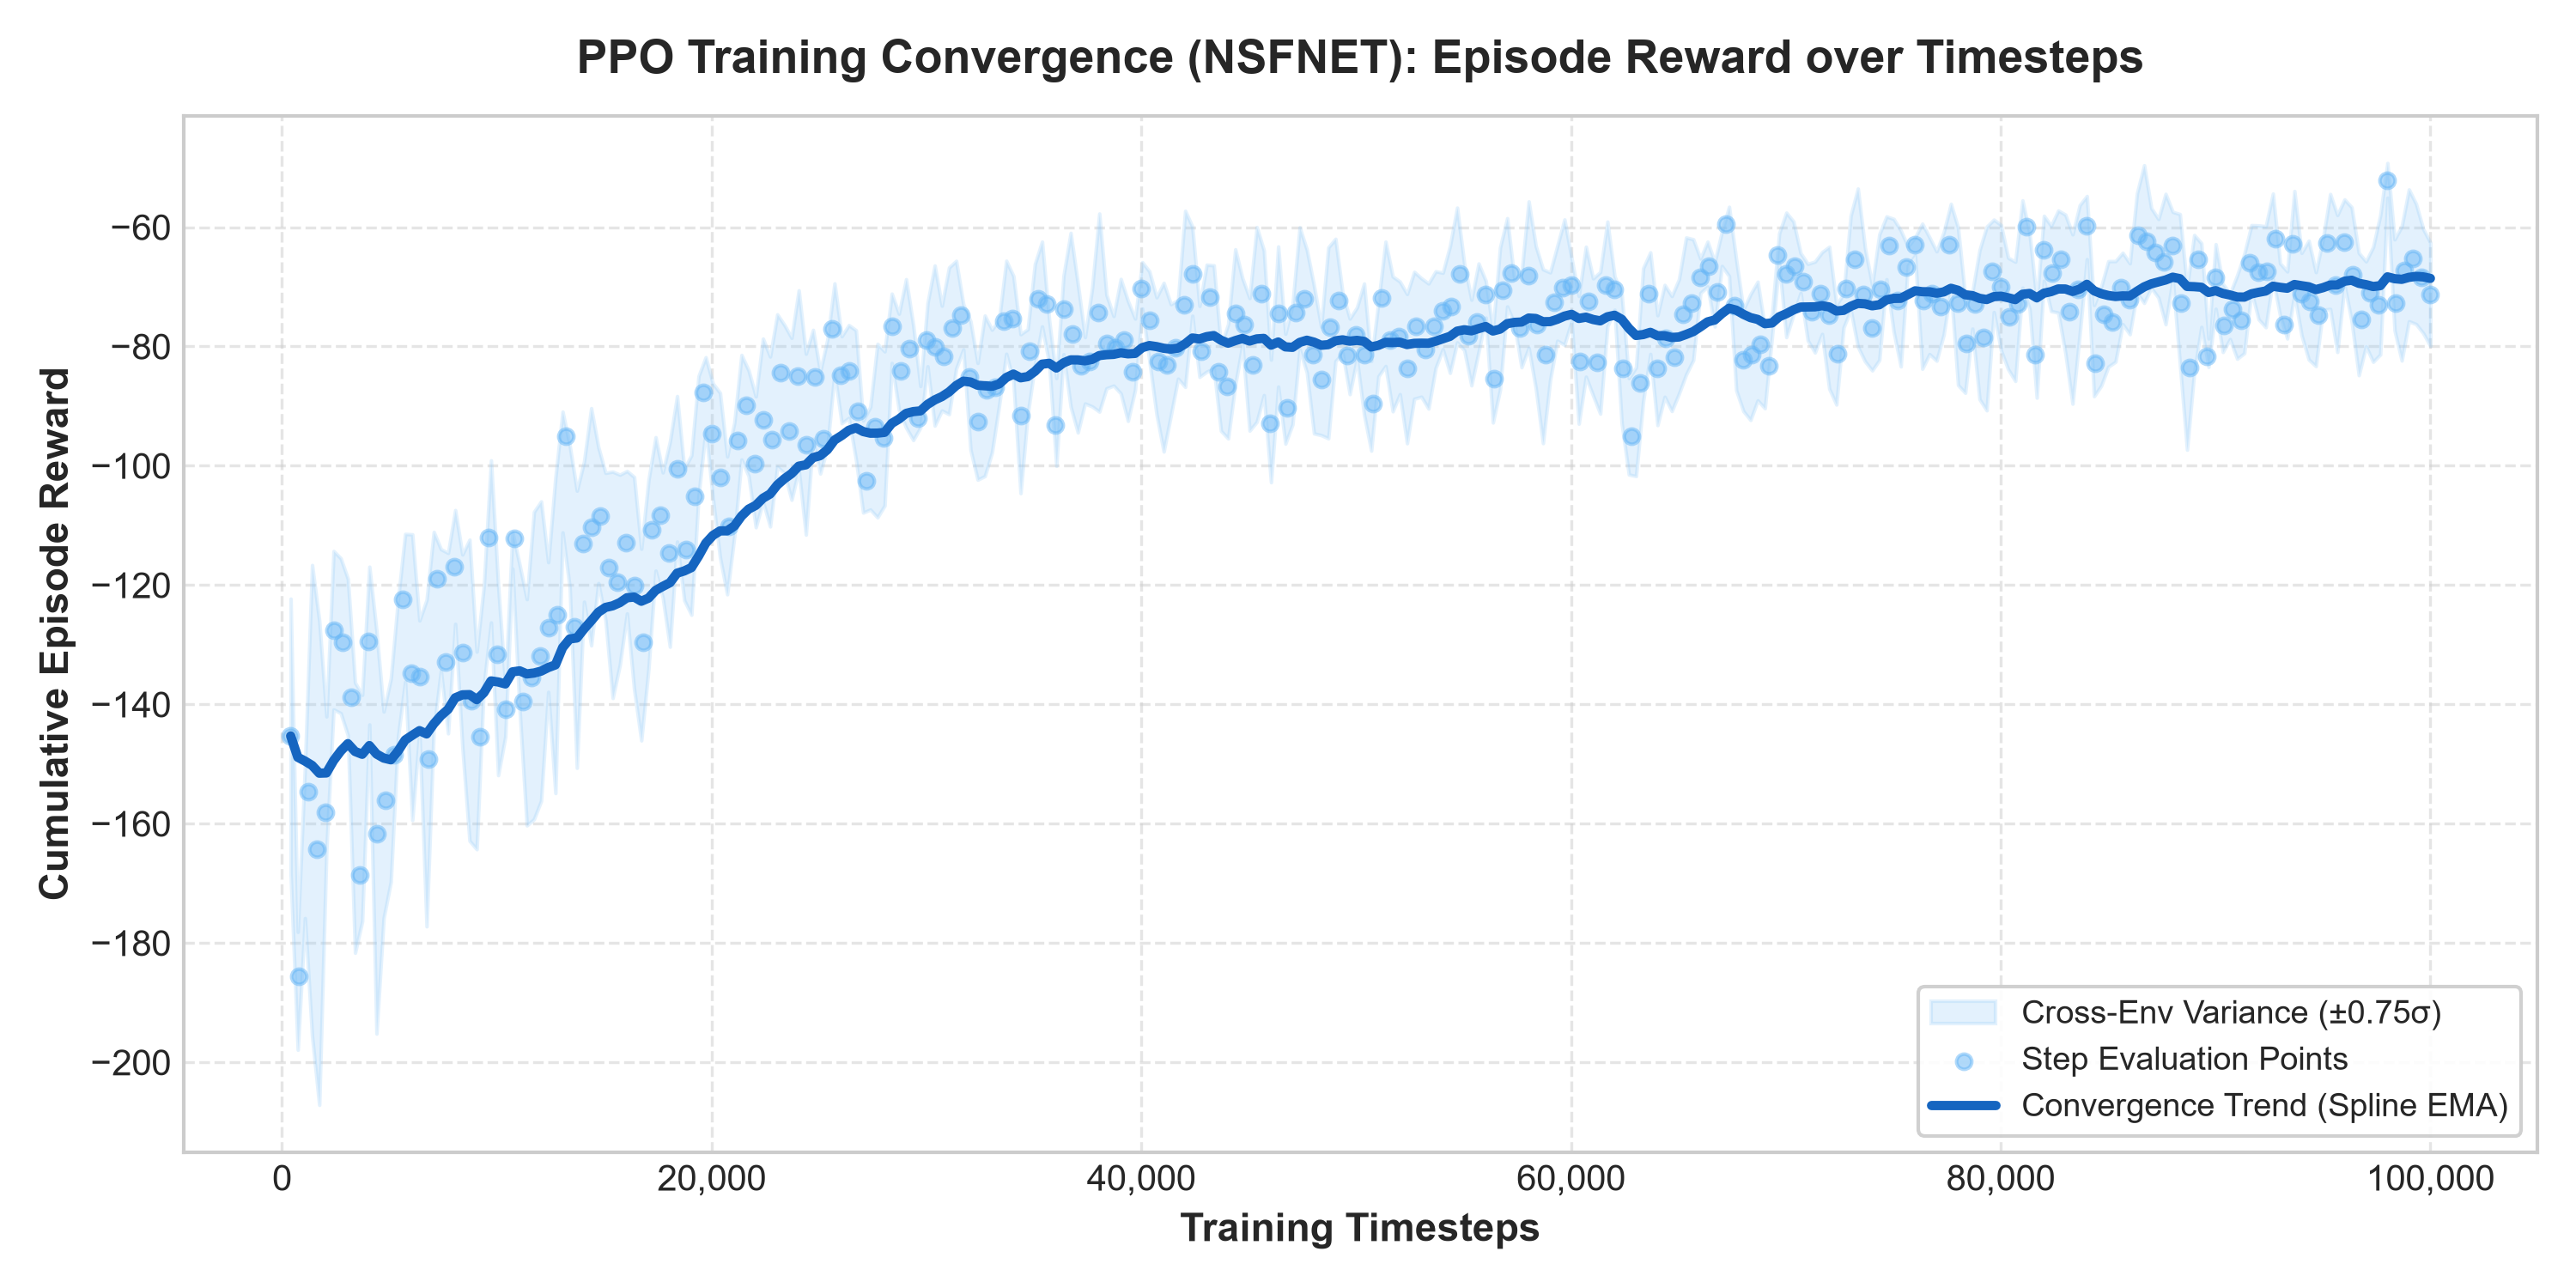
\includegraphics[width=\textwidth]{figures/training_nsfnet.png}
        \caption{NSFNET (100k bước)}
    \end{subfigure}\hfill
    \begin{subfigure}[b]{0.32\textwidth}
        \centering
        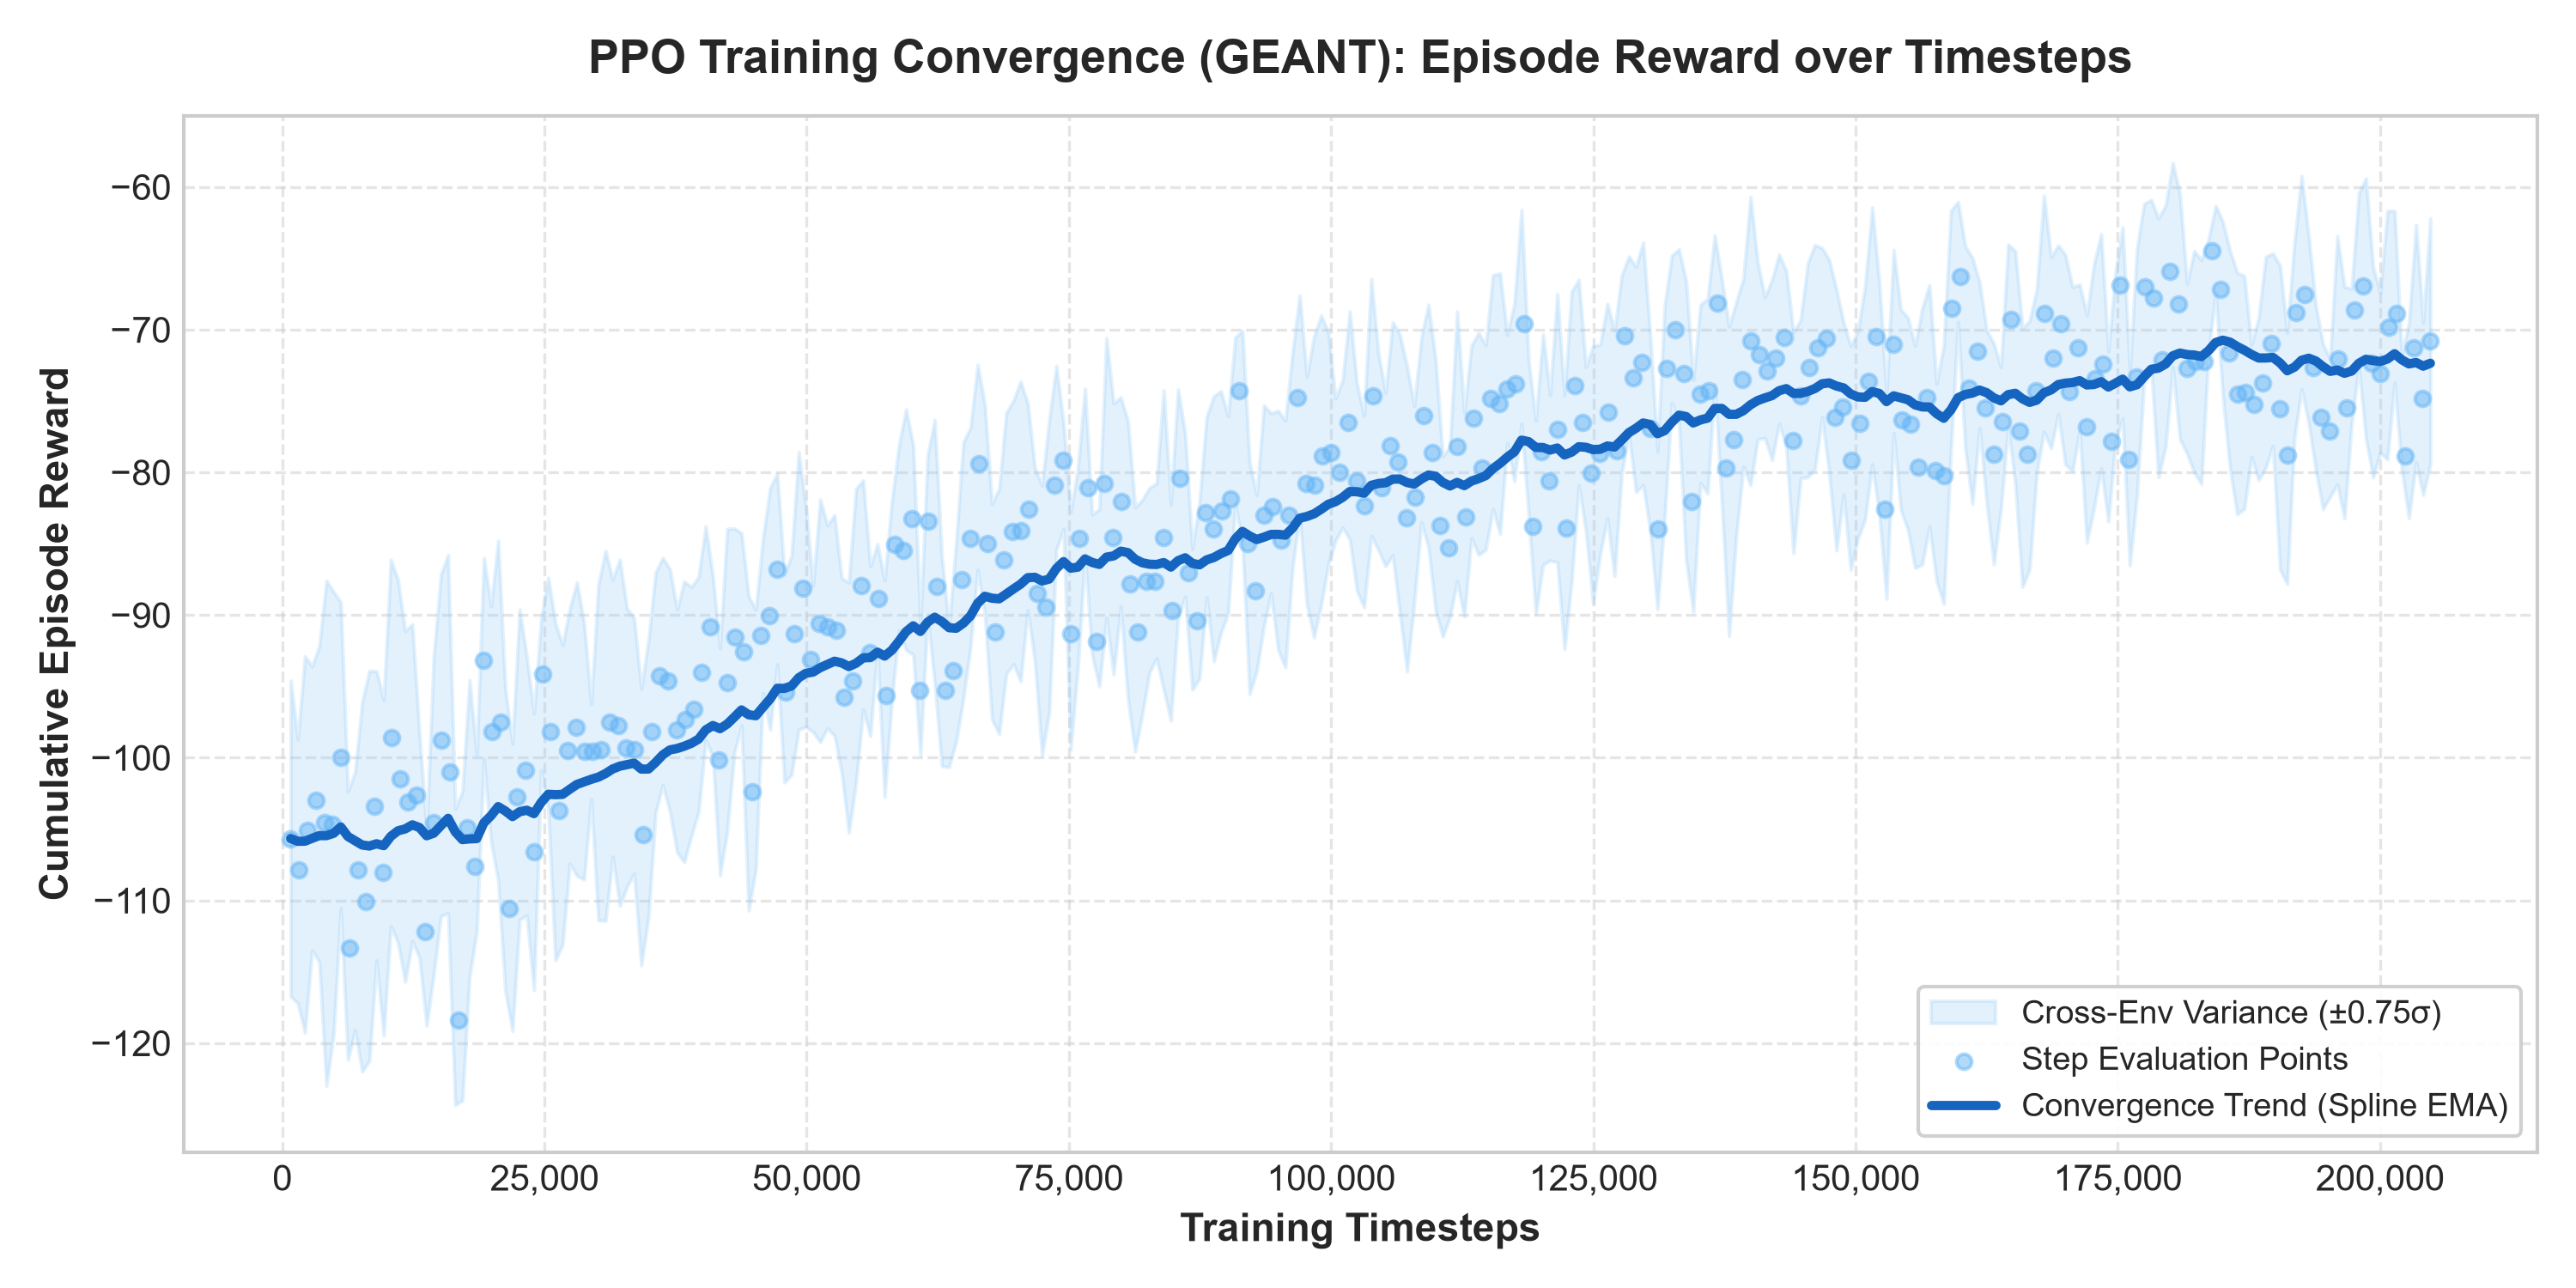
\includegraphics[width=\textwidth]{figures/training_geant.png}
        \caption{GÉANT (204.8k bước)}
    \end{subfigure}\hfill
    \begin{subfigure}[b]{0.32\textwidth}
        \centering
        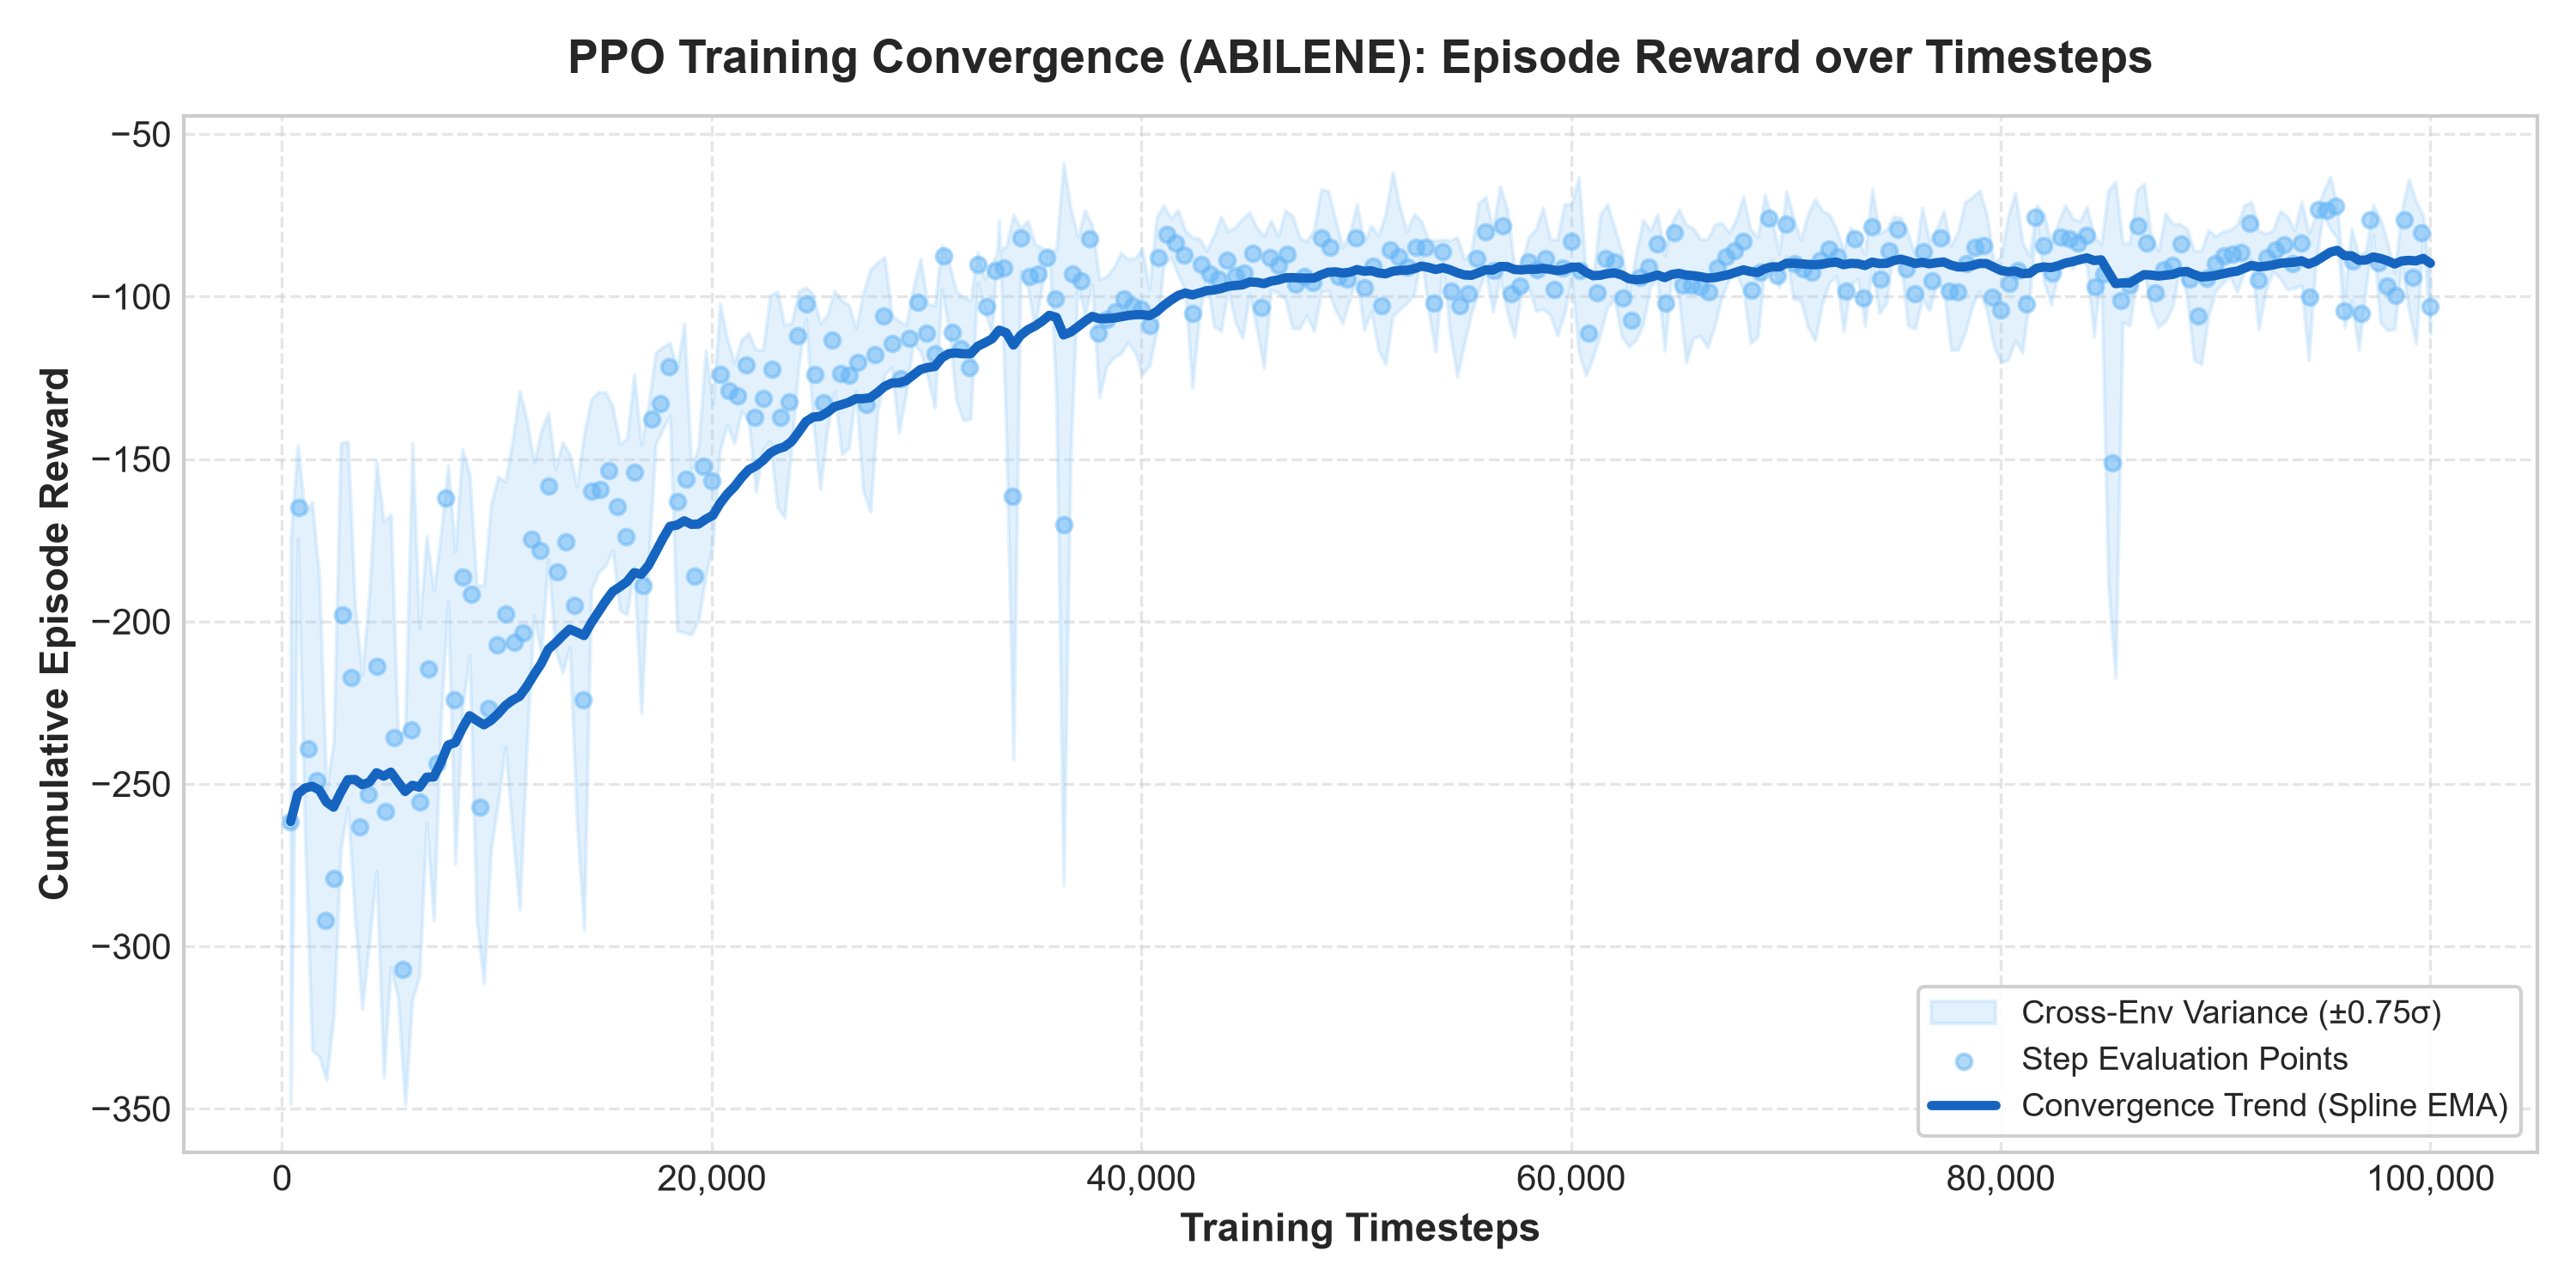
\includegraphics[width=\textwidth]{figures/training_abilene.png}
        \caption{Abilene (100k bước)}
    \end{subfigure}
    \caption{\textit{Đồ thị hội tụ phần thưởng huấn luyện (Episode Reward) của mô hình RecurrentPPO trên 3 mạng.}}
    \label{fig:training_all}
\end{figure}

\clearpage

\subsection*{Đánh giá thực nghiệm Trường hợp 1: Mạng NSFNET (14 nút, 42 liên kết)}
Đối sánh đa chính sách trên mạng NSFNET qua 6 kịch bản thực nghiệm (Bảng \ref{tab:nsfnet_summary} và Hình \ref{fig:nsfnet_all}):

\begin{table}[H]
\centering
\caption{\textit{Bảng tổng hợp đối sánh định lượng trên mạng NSFNET: OSPF-SPF và Tác tử Nội miền (In-Domain FL-DRL) qua 6 kịch bản.}}
\label{tab:nsfnet_summary}
\footnotesize
\setlength{\tabcolsep}{6pt}
\renewcommand{\arraystretch}{0.95}
\begin{tabular*}{\textwidth}{@{\extracolsep{\fill}} l l c c c @{}}
\toprule
\textbf{Kịch bản} & \textbf{Chính sách} & \textbf{MLU TB (Đỉnh)} & \textbf{Độ trễ (ms)} & \textbf{Mất gói (\%)} \\
\midrule
\textbf{T1} (Chu kỳ) & OSPF-SPF & $0.727$ ($0.793$) & $9.30$ & $0.00\%$ \\
& In-Domain (FL-DRL) & $\mathbf{0.571}$ ($\mathbf{0.625}$) & $\mathbf{8.01}$ & $0.00\%$ \\
\midrule
\textbf{T2} (Đột biến) & OSPF-SPF & $0.776$ ($1.255$) & $10.59$ & $2.38\%$ \\
& In-Domain (FL-DRL) & $\mathbf{0.623}$ ($\mathbf{1.151}$) & $\mathbf{8.47}$ & $\mathbf{0.89\%}$ \\
\midrule
\textbf{T3} (Tăng tải) & OSPF-SPF & $0.914$ ($1.142$) & $18.53$ & $18.46\%$ \\
& In-Domain (FL-DRL) & $\mathbf{0.717}$ ($\mathbf{0.901}$) & $\mathbf{8.01}$ & $\mathbf{0.31\%}$ \\
\midrule
\textbf{T4} (Dồn tải) & OSPF-SPF & $0.786$ ($1.950$) & $11.08$ & $2.50\%$ \\
& In-Domain (FL-DRL) & $\mathbf{0.637}$ ($\mathbf{1.950}$) & $\mathbf{9.95}$ & $2.50\%$ \\
\midrule
\textbf{T5} (Đứt link) & OSPF-SPF & $0.934$ ($1.150$) & $22.15$ & $35.99\%$ \\
& In-Domain (FL-DRL) & $\mathbf{0.820}$ ($\mathbf{1.051}$) & $\mathbf{14.35}$ & $\mathbf{13.17\%}$ \\
\midrule
\textbf{T6} (Lệch pha) & OSPF-SPF & $0.772$ ($1.473$) & $18.42$ & $15.60\%$ \\
& In-Domain (FL-DRL) & $\mathbf{0.607}$ ($\mathbf{1.188}$) & $\mathbf{18.24}$ & $\mathbf{14.17\%}$ \\
\bottomrule
\end{tabular*}
\end{table}

\begin{itemize}[leftmargin=1.5em, itemsep=0pt, parsep=0pt, topsep=2pt]
    \item \textbf{Diễn biến MLU (Hình \ref{fig:nsfnet_all}a):} Ở chu kỳ danh định T1, OSPF có MLU trung bình $0.727$ (đỉnh $0.793$). Tác tử In-Domain phân tán các luồng voi sang tuyến phụ, hạ MLU xuống $0.571$ (đỉnh $0.625$, giảm $21.5\%$). Khi mạng chịu quá tải lũy tiến $+50\%$ ở kịch bản T3, OSPF bị dồn nghẽn cục bộ nghiêm trọng ($\text{MLU} = 0.914$, đỉnh $1.142$); trong khi đó, tác tử In-Domain kiểm soát tải tối ưu ở mức $0.717$ (đỉnh $0.901$, luôn duy trì dưới ngưỡng nghẽn).
    \item \textbf{Độ trễ trung bình (Hình \ref{fig:nsfnet_all}b):} Trên mạng NSFNET, chiều dài sợi quang giữa các cặp nút chênh lệch lớn. Tác tử In-Domain chọn tuyến đa chặng tối ưu trễ lan truyền, hạ trễ trung bình toàn mạng xuống $8.01$ ms (thấp hơn $9.30$ ms của OSPF). Khi xảy ra nghẽn nặng ở T3, hàng đợi OSPF phình to khiến trễ tăng vọt lên $18.53$ ms; tác tử In-Domain triệt tiêu nghẽn hàng đợi và duy trì trễ ổn định ở mức $8.01$ ms (giảm $56.8\%$).
    \item \textbf{Tỷ lệ mất gói (Hình \ref{fig:nsfnet_all}c):} Khi dồn tải và đứt cáp, OSPF chịu mất gói nặng: $18.46\%$ ở T3, $35.99\%$ ở T5 và $15.60\%$ ở T6. Tác tử In-Domain cắt giảm tới $98.3\%$ lượng gói mất ở T3 (còn $0.31\%$), giảm $63.4\%$ mất gói khi đứt cáp ở T5 (còn $13.17\%$) và duy trì tỷ lệ mất gói thấp nhất ở T6 ($14.17\%$).
\end{itemize}

\clearpage

\begin{figure}[p]
    \centering
    \begin{subfigure}[b]{0.96\textwidth}
        \centering
        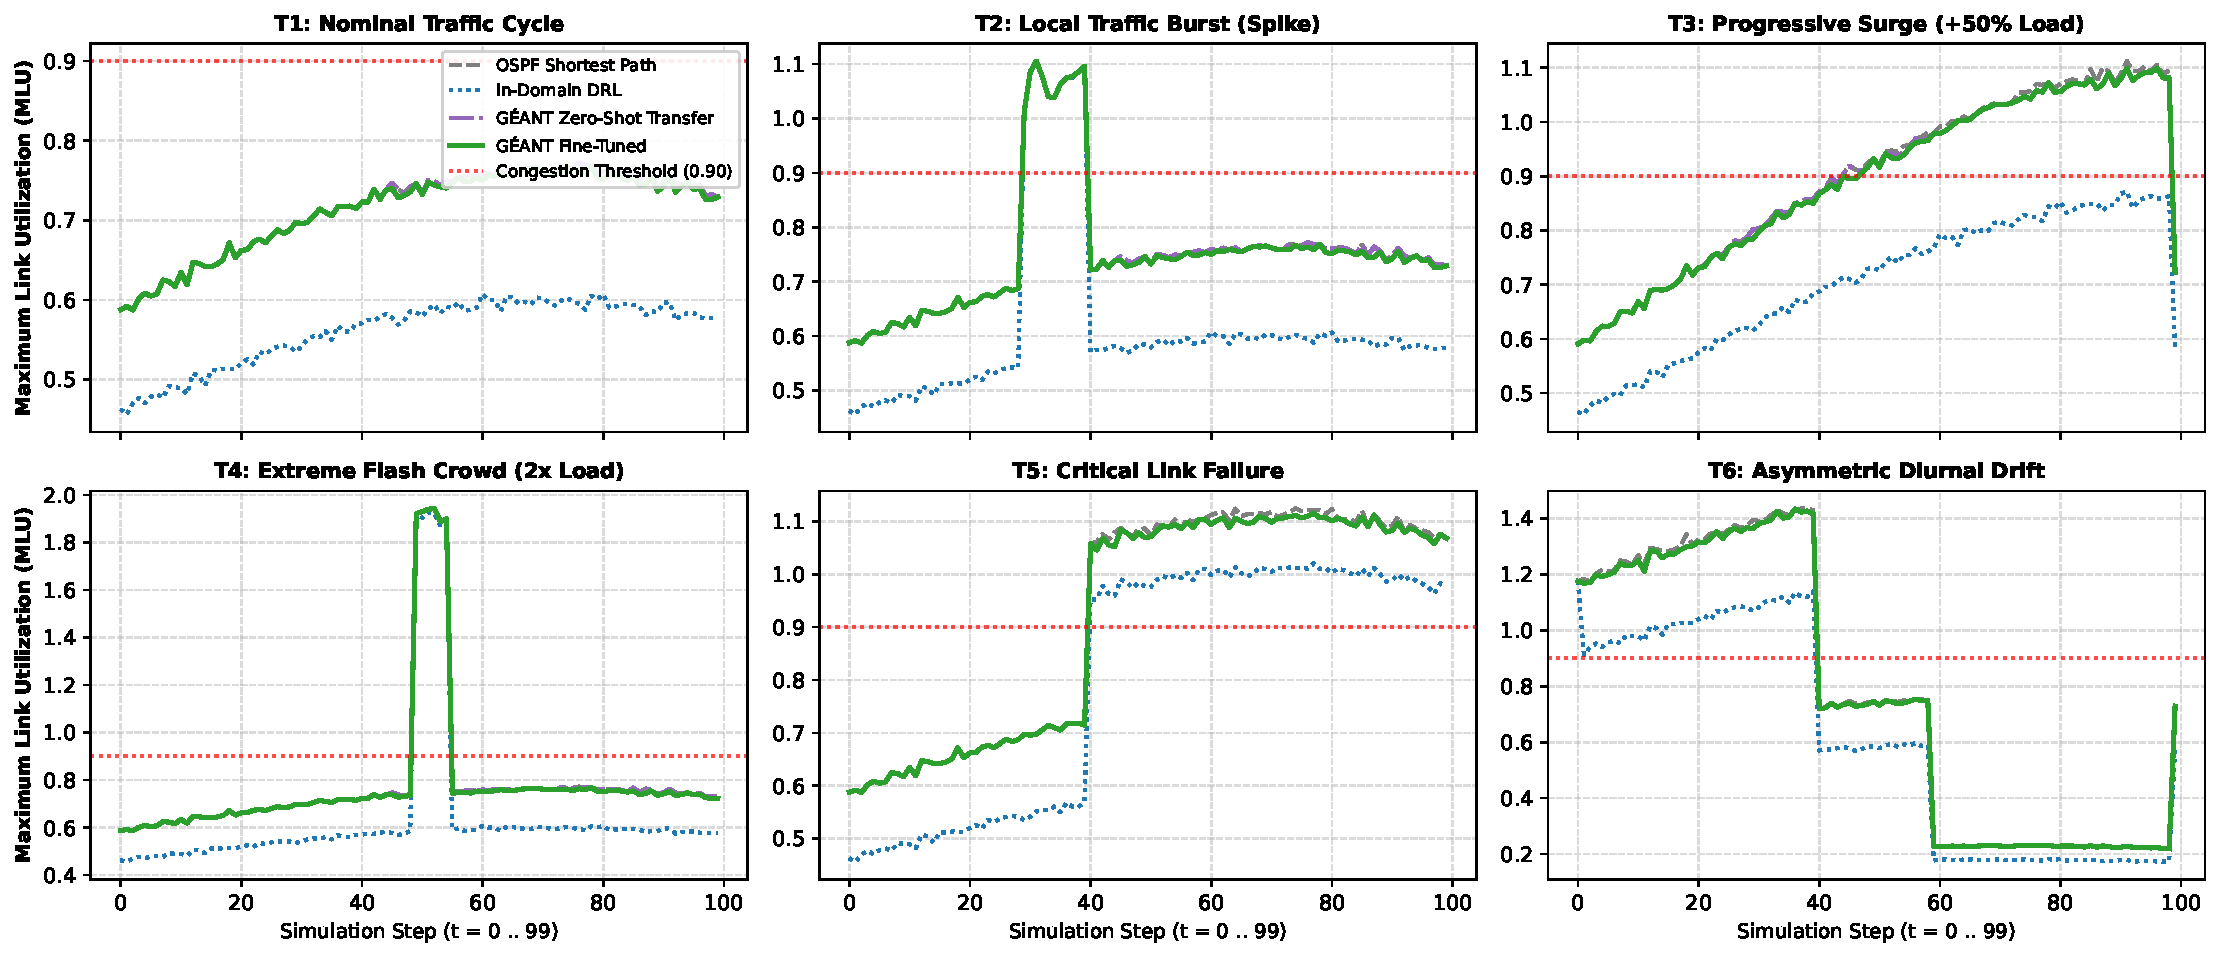
\includegraphics[width=\textwidth]{figures/overview_nsfnet_mlu.pdf}
        \caption{Mức sử dụng cực đại (MLU)}
    \end{subfigure}
    \vspace{0.15cm}
    \begin{subfigure}[b]{0.96\textwidth}
        \centering
        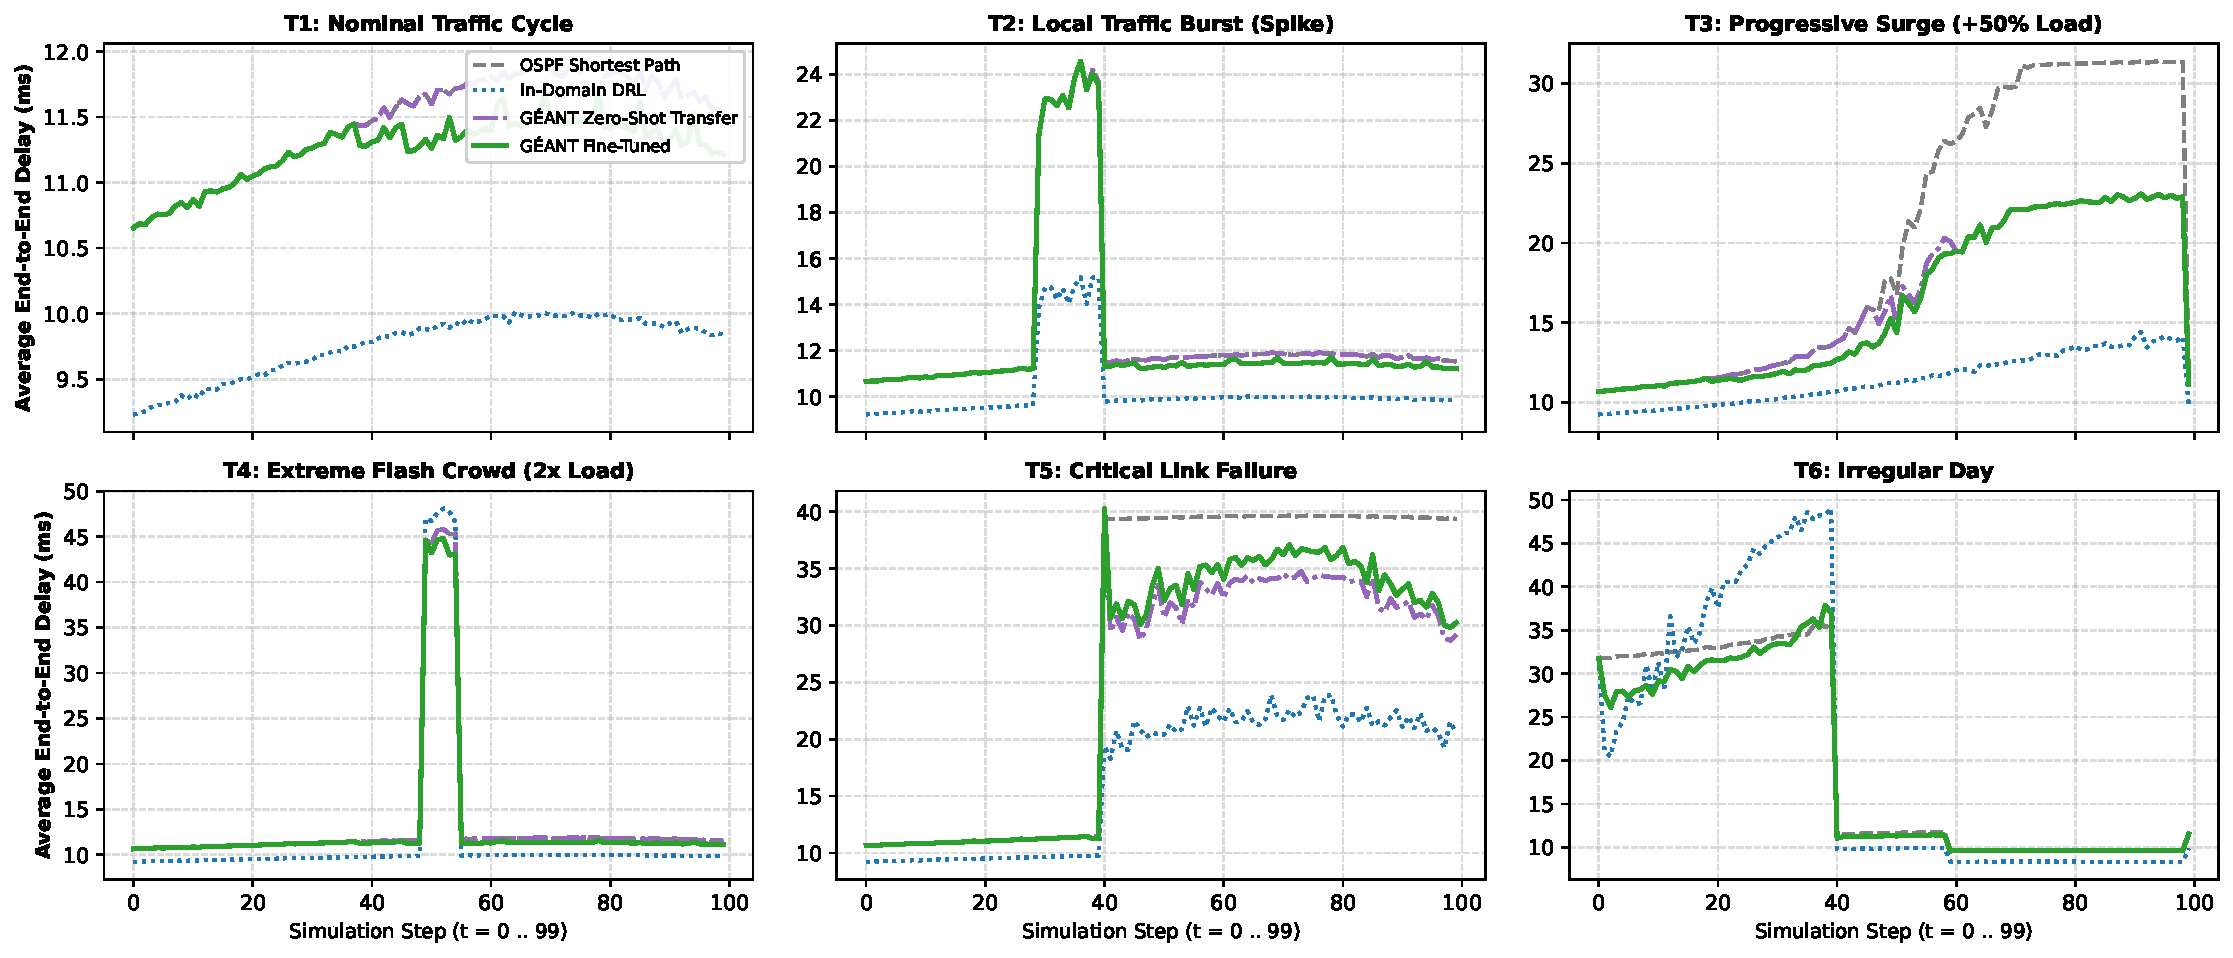
\includegraphics[width=\textwidth]{figures/overview_nsfnet_delay.pdf}
        \caption{Độ trễ trung bình (ms)}
    \end{subfigure}
    \vspace{0.15cm}
    \begin{subfigure}[b]{0.96\textwidth}
        \centering
        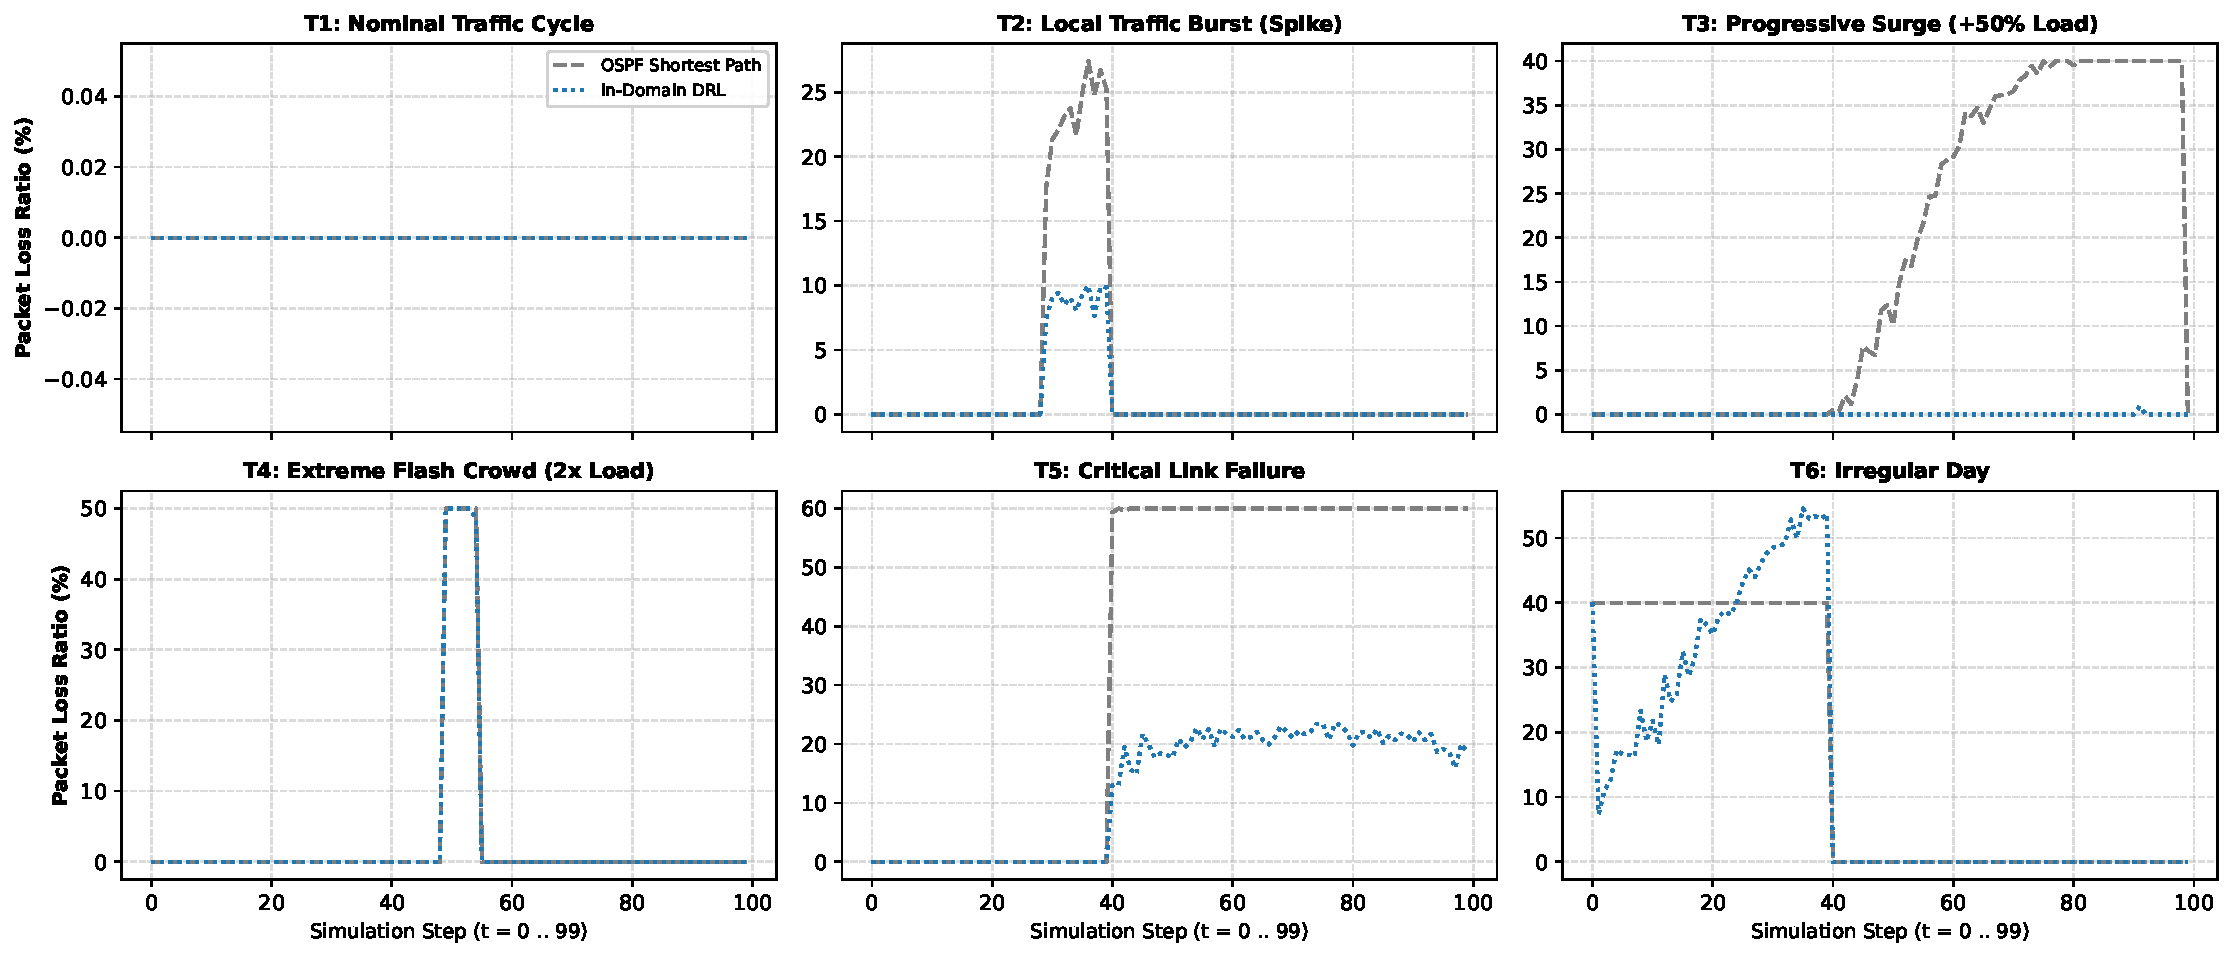
\includegraphics[width=\textwidth]{figures/overview_nsfnet_loss.pdf}
        \caption{Tỷ lệ mất gói (\%)}
    \end{subfigure}
    \caption{\textit{Toàn cảnh 6 kịch bản trên mạng NSFNET: MLU, Độ trễ và Tỷ lệ Mất gói (Lưới 2x3 vector chuẩn).}}
    \label{fig:nsfnet_all}
\end{figure}

\clearpage

\subsection*{Đánh giá thực nghiệm Trường hợp 2: Mạng GÉANT (22 nút, 72 liên kết)}
Phân tích kết quả định lượng chi tiết trên mạng lõi GÉANT (Bảng \ref{tab:geant_summary} và Hình \ref{fig:geant_all}):

\begin{table}[H]
\centering
\caption{\textit{Bảng tổng hợp đối sánh định lượng trên mạng GÉANT qua 6 kịch bản (Trung bình qua 3 random seeds).}}
\label{tab:geant_summary}
\footnotesize
\setlength{\tabcolsep}{4pt}
\renewcommand{\arraystretch}{0.88}
\begin{tabular*}{\textwidth}{@{\extracolsep{\fill}} l l c c c @{}}
\toprule
\textbf{Kịch bản} & \textbf{Chính sách} & \textbf{MLU TB (Đỉnh)} & \textbf{Độ trễ (ms)} & \textbf{Mất gói (\%)} \\
\midrule
\textbf{T1} (Chu kỳ) & OSPF-SPF & $0.727$ ($0.796$) & $\mathbf{10.40}$ & $0.00\%$ \\
& Proactive FL-DRL & $\mathbf{0.598}$ ($\mathbf{0.657}$) & $10.70$ & $0.00\%$ \\
\midrule
\textbf{T2} (Đột biến) & OSPF-SPF & $0.776$ ($1.255$) & $12.62$ & $3.97\%$ \\
& Proactive FL-DRL & $\mathbf{0.638}$ ($\mathbf{1.031}$) & $\mathbf{10.95}$ & $\mathbf{0.55\%}$ \\
\midrule
\textbf{T3} (Tăng tải) & OSPF-SPF & $0.914$ ($1.142$) & $19.23$ & $16.75\%$ \\
& Proactive FL-DRL & $\mathbf{0.694}$ ($\mathbf{0.835}$) & $\mathbf{10.76}$ & $\mathbf{0.00\%}$ \\
\midrule
\textbf{T4} (Dồn tải) & OSPF-SPF & $0.780$ ($1.883$) & $12.32$ & $3.00\%$ \\
& Proactive FL-DRL & $\mathbf{0.645}$ ($\mathbf{1.632}$) & $\mathbf{12.06}$ & $\mathbf{2.20\%}$ \\
\midrule
\textbf{T5} (Đứt link) & OSPF-SPF & $0.751$ ($0.836$) & $\mathbf{10.88}$ & $0.00\%$ \\
& Proactive FL-DRL & $\mathbf{0.721}$ ($\mathbf{0.872}$) & $11.50$ & $0.03\%$ \\
\midrule
\textbf{T6} (Lệch pha) & OSPF-SPF & $0.771$ ($1.478$) & $26.09$ & $23.34\%$ \\
& Proactive FL-DRL & $\mathbf{0.588}$ ($\mathbf{1.070}$) & $\mathbf{15.30}$ & $\mathbf{8.20\%}$ \\
\bottomrule
\end{tabular*}
\end{table}

\begin{itemize}[leftmargin=1.5em, itemsep=0pt, parsep=0pt, topsep=2pt]
    \item \textbf{Diễn biến MLU (Hình \ref{fig:geant_all}a):} Nhờ cấu trúc đồ thị dày và dung lượng lớn (2.5 Gbps), tác tử phân bổ luồng hiệu quả, giảm $17.7\%$ MLU ở kịch bản T1 ($0.598$ so với $0.727$ của OSPF). Ở các kịch bản áp lực cao T2, T3 và T4, MLU của tác tử duy trì ở mức an toàn dưới ngưỡng 0.90 (ở T3 hạ từ $0.914$ xuống $0.694$, giá trị đỉnh hạ từ $1.142$ xuống $0.835$).
    \item \textbf{Độ trễ trung bình (Hình \ref{fig:geant_all}b):} Ở kịch bản danh định T1, OSPF đạt trễ lan truyền thấp nhất ($10.40$ ms) do sử dụng tuyến ngắn nhất, trong khi tác tử có độ trễ tương đương ($10.70$ ms). Khi mạng chịu tải cao ở T3 và T6, độ trễ của OSPF tăng lên $19.23$ ms và $26.09$ ms; trong khi đó, tác tử duy trì độ trễ ổn định ở mức $10.76$ ms (T3) và $15.30$ ms (giảm $41.4\%$ so với OSPF ở T6).
    \item \textbf{Tỷ lệ mất gói (Hình \ref{fig:geant_all}c):} OSPF chịu ảnh hưởng nghẽn với tỷ lệ mất gói $3.97\%$ ở T2, $16.75\%$ ở T3 và $23.34\%$ ở T6. Tác tử FL-DRL giảm tỷ lệ mất gói xuống $0.55\%$ ở T2, triệt tiêu mất gói ở kịch bản T3 về mức $0.00\%$, và giảm tỷ lệ mất gói ở T6 xuống $8.20\%$ (giảm $64.9\%$ so với OSPF).
\end{itemize}

\clearpage

\begin{figure}[p]
    \centering
    \begin{subfigure}[b]{0.96\textwidth}
        \centering
        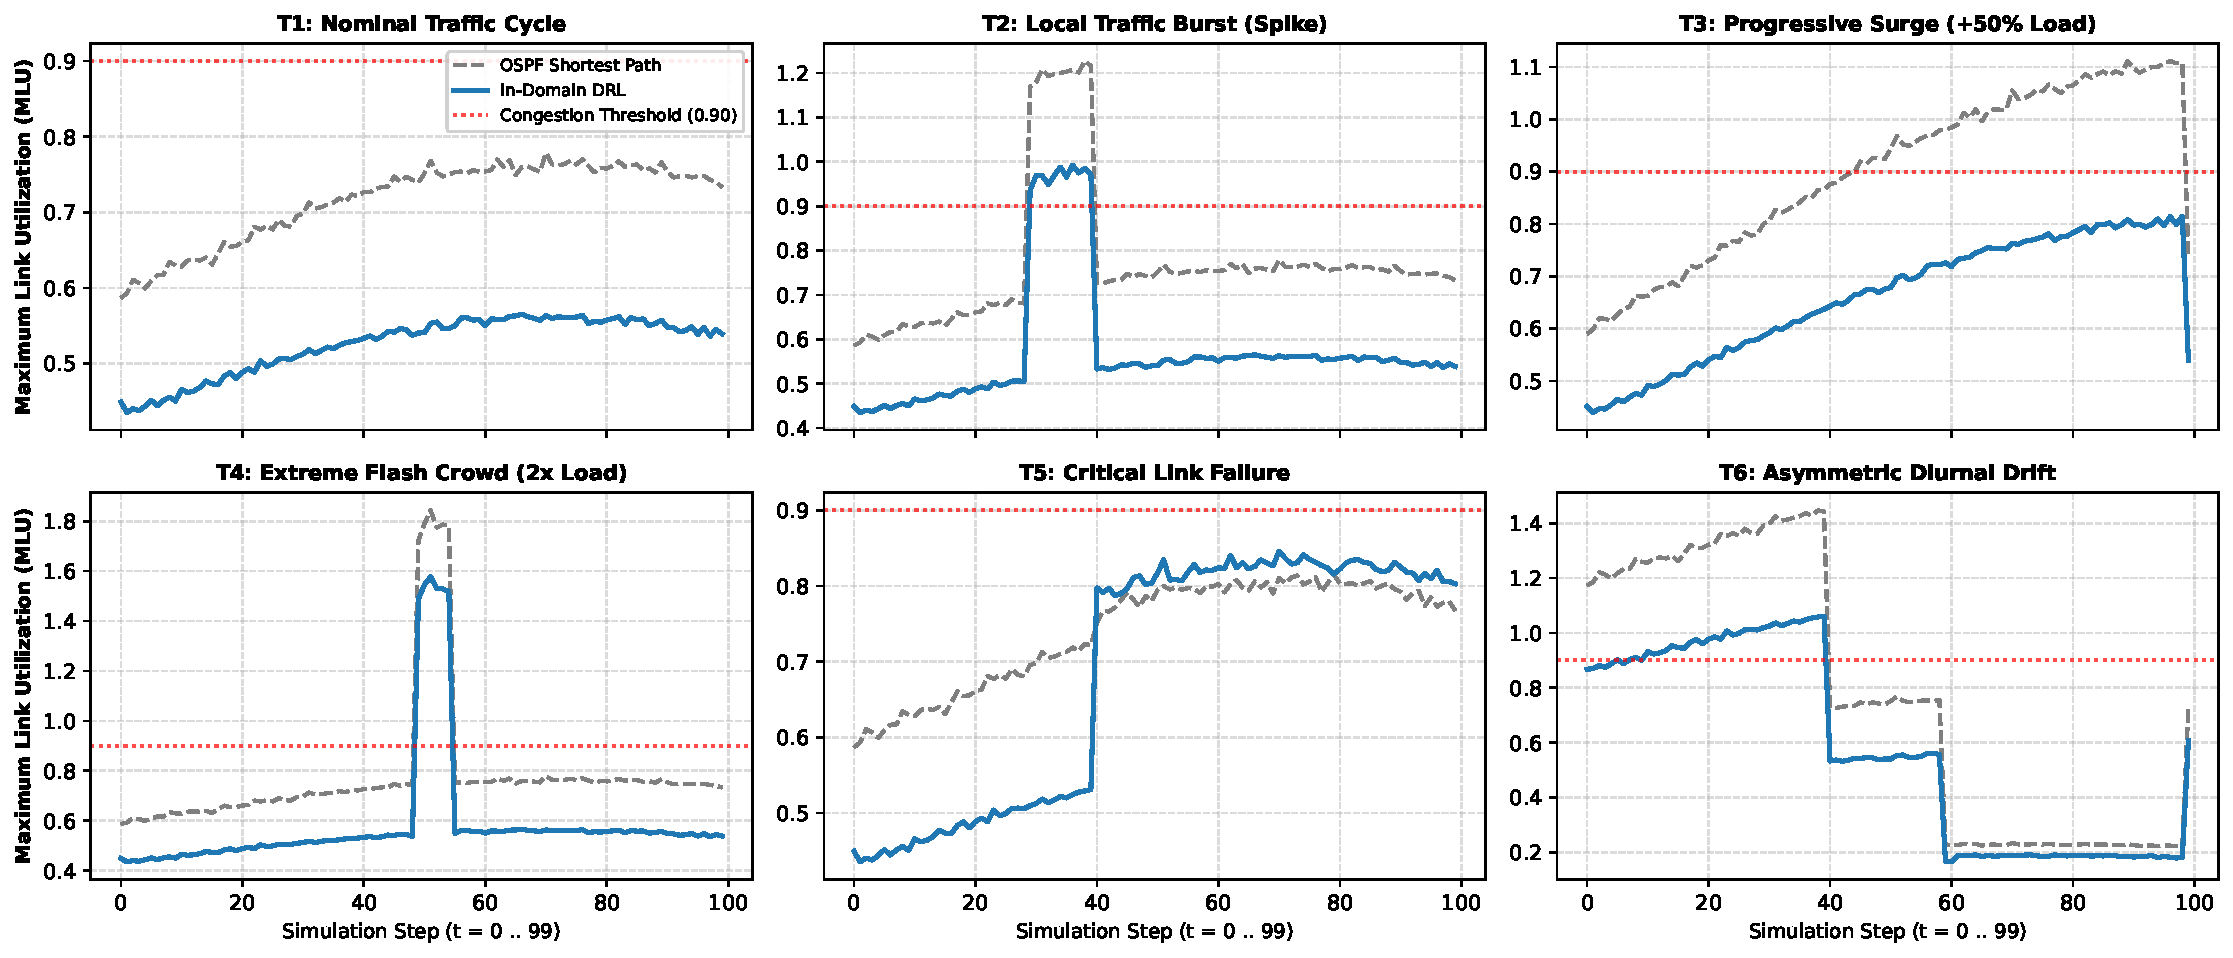
\includegraphics[width=\textwidth]{figures/overview_geant_mlu.pdf}
        \caption{Mức sử dụng cực đại (MLU)}
    \end{subfigure}
    \vspace{0.15cm}
    \begin{subfigure}[b]{0.96\textwidth}
        \centering
        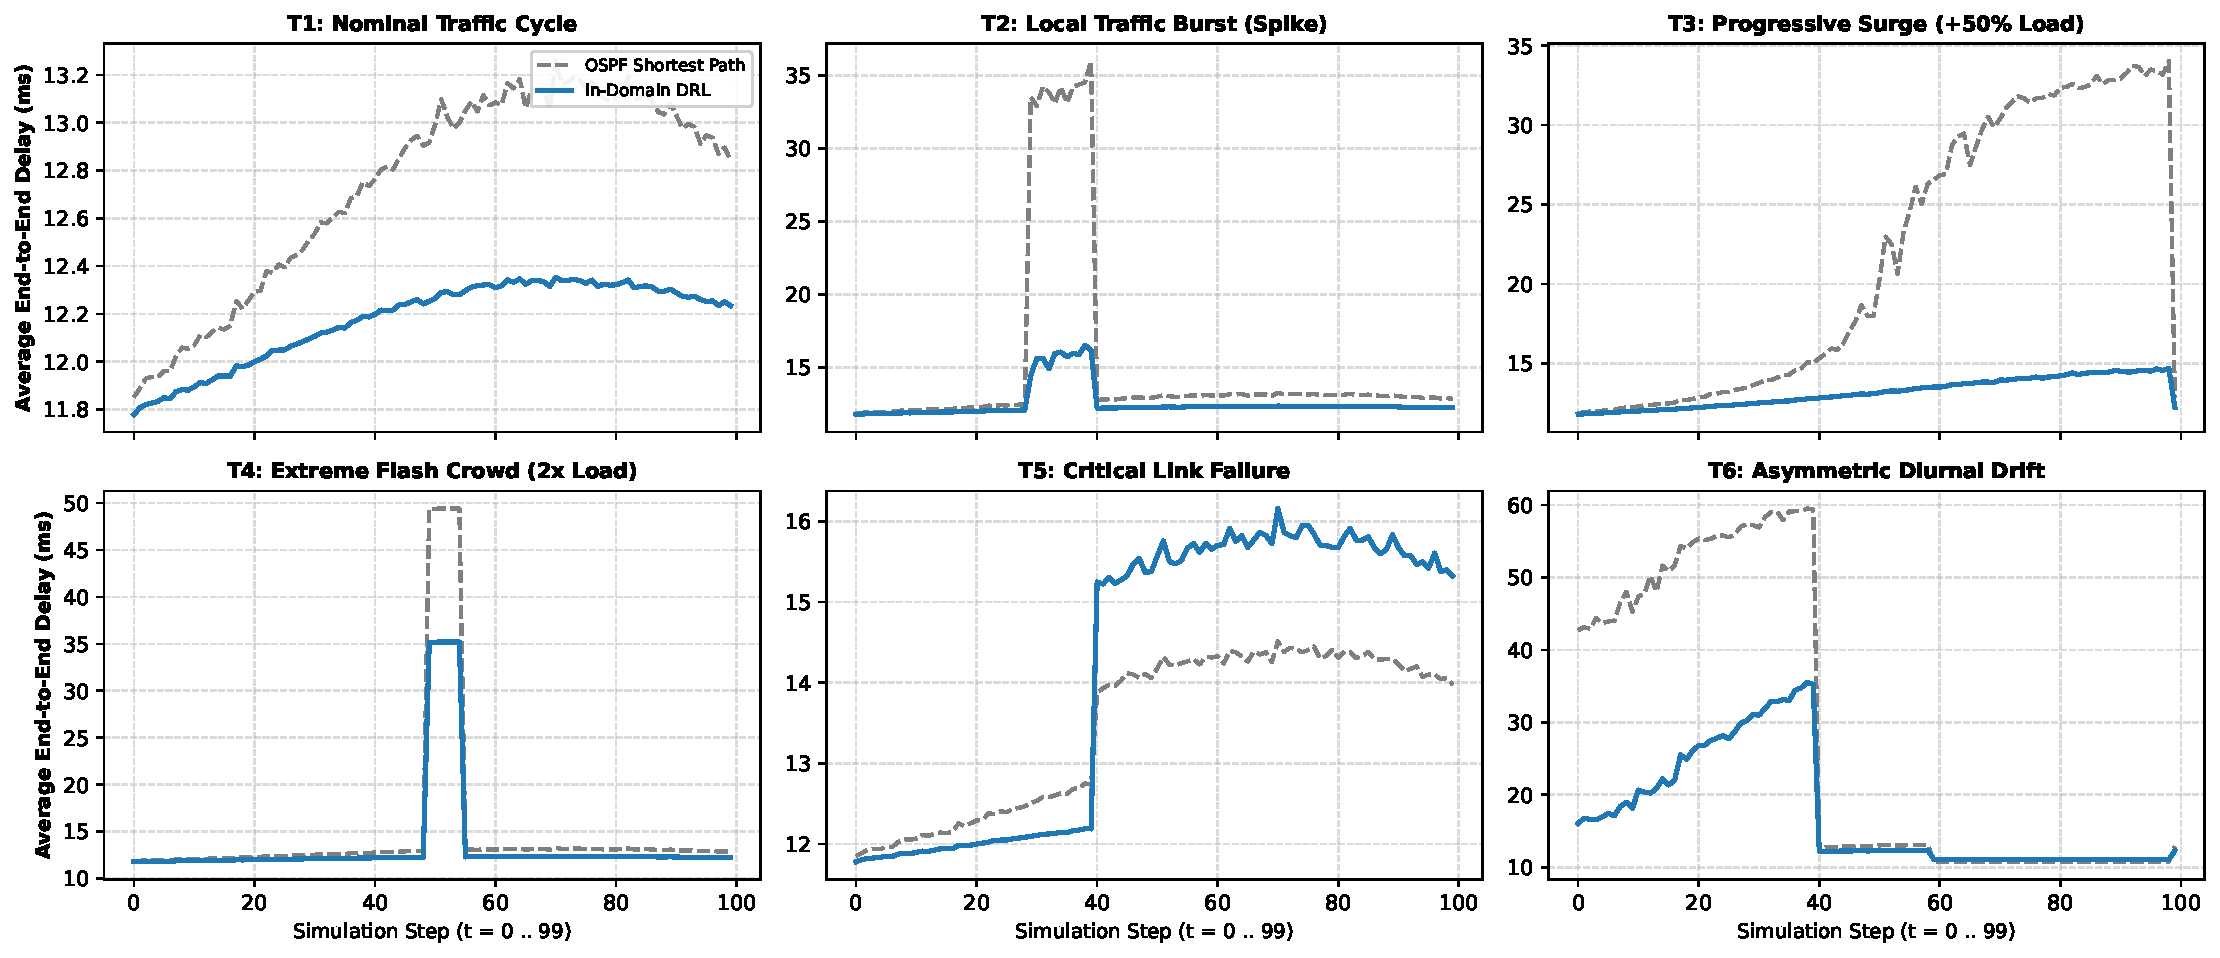
\includegraphics[width=\textwidth]{figures/overview_geant_delay.pdf}
        \caption{Độ trễ trung bình (ms)}
    \end{subfigure}
    \vspace{0.15cm}
    \begin{subfigure}[b]{0.96\textwidth}
        \centering
        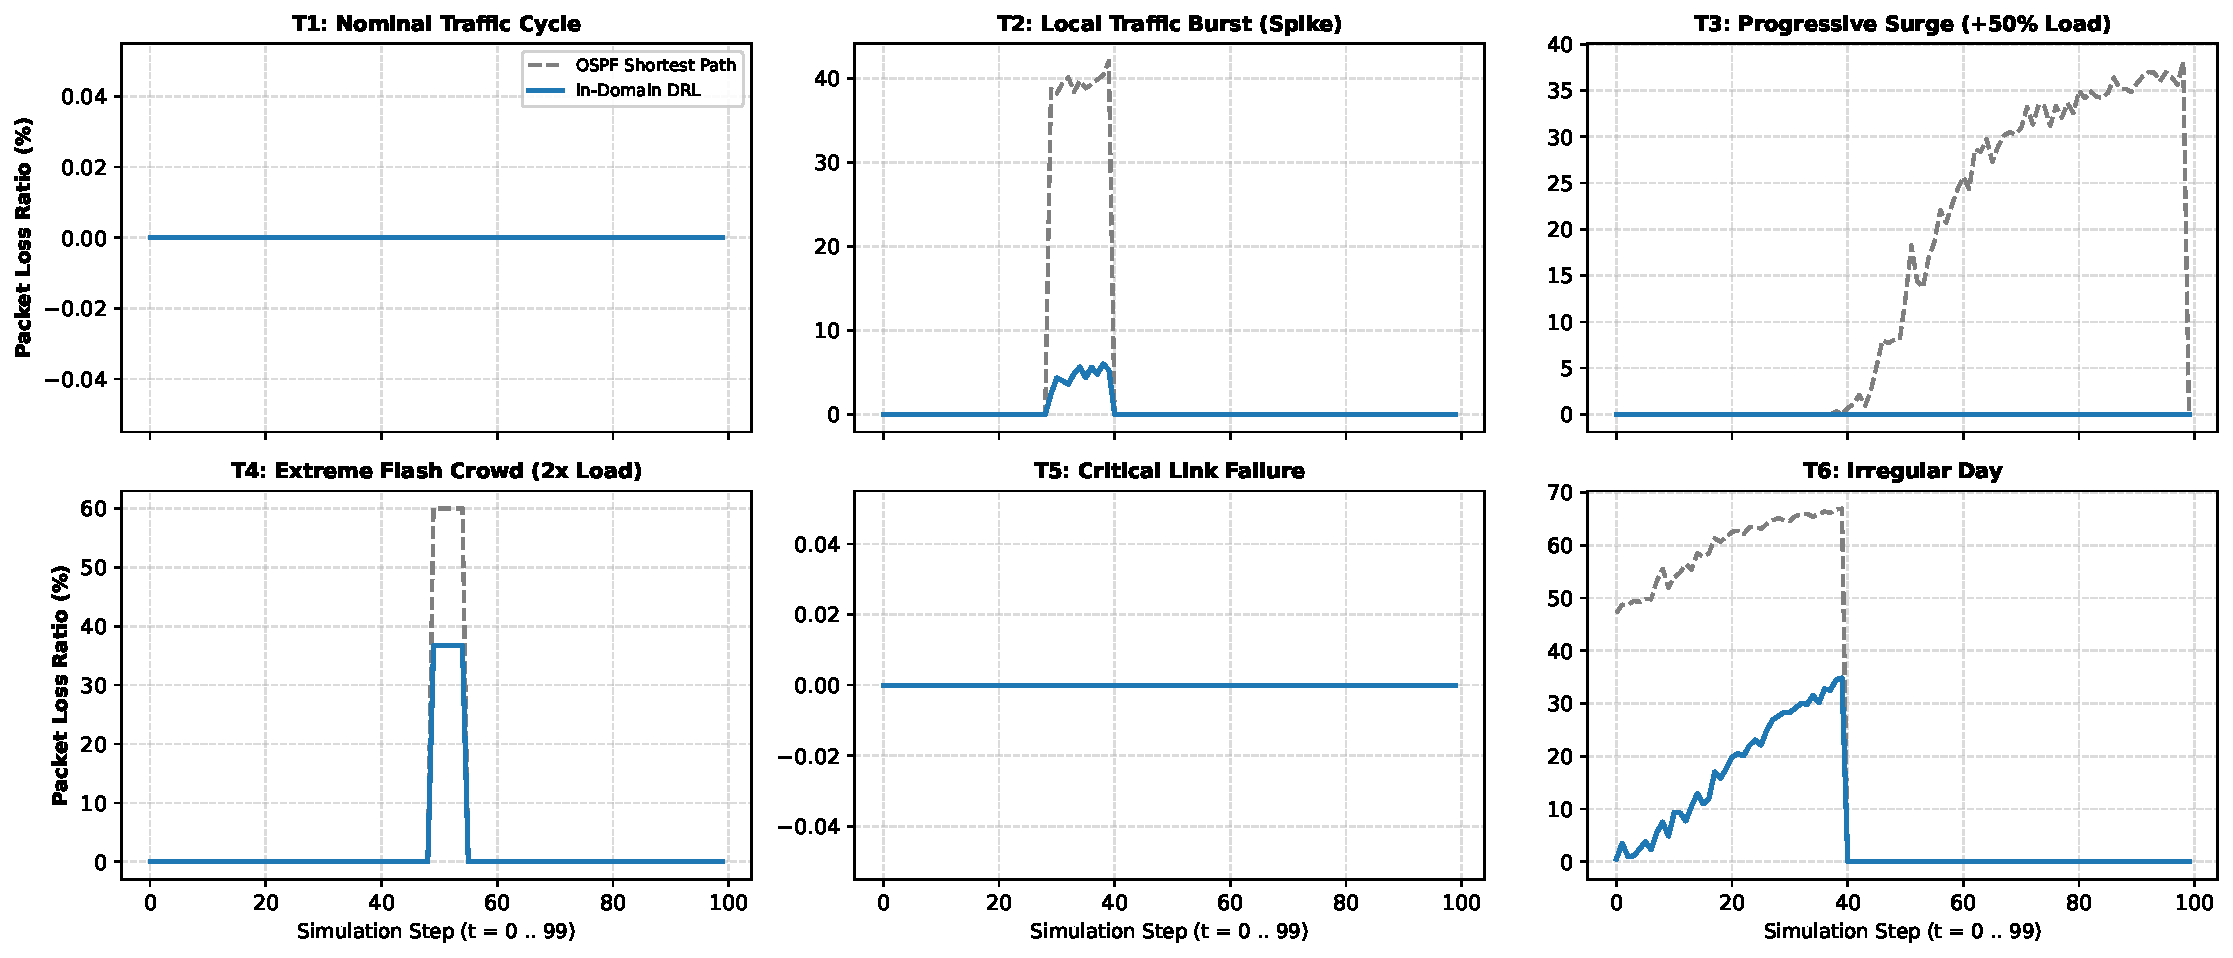
\includegraphics[width=\textwidth]{figures/overview_geant_loss.pdf}
        \caption{Tỷ lệ mất gói (\%)}
    \end{subfigure}
    \caption{\textit{Toàn cảnh 6 kịch bản trên mạng GÉANT: MLU, Độ trễ và Tỷ lệ Mất gói (Lưới 2x3 vector chuẩn).}}
    \label{fig:geant_all}
\end{figure}

\clearpage

\subsection*{Đánh giá thực nghiệm Trường hợp 3: Mạng Abilene (12 nút, 30 liên kết) - So sánh Đối đầu và Chuyển giao}
Đối sánh toàn diện giữa OSPF, Tác tử Nội miền (In-Domain), Tác tử Chuyển giao không mẫu (GEANT Transfer) và Tác tử Tinh chỉnh thích ứng (GEANT Finetuned) (Bảng \ref{tab:abilene_summary} và Hình \ref{fig:abilene_all}):

\begin{table}[H]
\centering
\caption{\textit{Bảng tổng hợp đối sánh định lượng trên mạng Abilene: OSPF, In-Domain, GEANT Transfer và GEANT Finetune.}}
\label{tab:abilene_summary}
\footnotesize
\setlength{\tabcolsep}{4pt}
\renewcommand{\arraystretch}{0.85}
\begin{tabular*}{\textwidth}{@{\extracolsep{\fill}} l l c c c @{}}
\toprule
\textbf{Kịch bản} & \textbf{Chính sách} & \textbf{MLU TB (Đỉnh)} & \textbf{Độ trễ (ms)} & \textbf{Mất gói (\%)} \\
\midrule
\textbf{T1} (Chu kỳ) & OSPF-SPF & $0.725$ ($0.790$) & $\mathbf{12.00}$ & $0.00\%$ \\
& In-Domain & $\mathbf{0.721}$ ($\mathbf{0.785}$) & $12.40$ & $0.00\%$ \\
& GEANT Transfer & $0.725$ ($0.790$) & $12.37$ & $0.00\%$ \\
& GEANT Finetuned & $0.722$ ($0.788$) & $12.93$ & $0.00\%$ \\
\midrule
\textbf{T2} (Đột biến) & OSPF-SPF & $0.789$ ($1.419$) & $\mathbf{14.00}$ & $4.36\%$ \\
& In-Domain & $\mathbf{0.787}$ ($1.435$) & $14.73$ & $4.58\%$ \\
& GEANT Transfer & $0.789$ ($1.419$) & $14.59$ & $4.36\%$ \\
& GEANT Finetuned & $0.788$ ($1.419$) & $15.15$ & $\mathbf{4.33\%}$ \\
\midrule
\textbf{T3} (Tăng tải) & OSPF-SPF & $0.912$ ($1.136$) & $26.72$ & $21.80\%$ \\
& In-Domain & $\mathbf{0.906}$ ($1.134$) & $23.09$ & $17.64\%$ \\
& GEANT Transfer & $0.912$ ($1.136$) & $25.67$ & $20.66\%$ \\
& GEANT Finetuned & $0.907$ ($\mathbf{1.127}$) & $\mathbf{20.35}$ & $\mathbf{12.26\%}$ \\
\midrule
\textbf{T4} (Dồn tải) & OSPF-SPF & $0.787$ ($2.000$) & $\mathbf{14.00}$ & $\mathbf{3.67\%}$ \\
& In-Domain & $\mathbf{0.783}$ ($2.000$) & $14.40$ & $\mathbf{3.67\%}$ \\
& GEANT Transfer & $0.787$ ($2.000$) & $14.37$ & $\mathbf{3.67\%}$ \\
& GEANT Finetuned & $0.785$ ($2.000$) & $14.93$ & $\mathbf{3.67\%}$ \\
\midrule
\textbf{T5} (Đứt link) & OSPF-SPF & $1.014$ ($1.294$) & $42.00$ & $32.00\%$ \\
& In-Domain & $\mathbf{1.012}$ ($1.294$) & $43.08$ & $32.00\%$ \\
& GEANT Transfer & $1.014$ ($1.294$) & $\mathbf{41.93}$ & $32.00\%$ \\
& GEANT Finetuned & $1.014$ ($1.294$) & $42.01$ & $32.00\%$ \\
\midrule
\textbf{T6} (Lệch pha) & OSPF-SPF & $0.771$ ($1.462$) & $43.97$ & $33.17\%$ \\
& In-Domain & $\mathbf{0.764}$ ($\mathbf{1.461}$) & $\mathbf{37.76}$ & $\mathbf{29.60\%}$ \\
& GEANT Transfer & $0.769$ ($1.462$) & $41.06$ & $30.47\%$ \\
& GEANT Finetuned & $0.767$ ($1.458$) & $39.71$ & $29.96\%$ \\
\bottomrule
\end{tabular*}
\end{table}

\begin{itemize}[leftmargin=1.5em, itemsep=0pt, parsep=0pt, topsep=2pt]
    \item \textbf{Cực tiểu lý thuyết độ trễ OSPF ở kịch bản T1:} Mạng Abilene có cấu trúc vành đai thưa thớt (12 nút, 30 liên kết); các đường rẽ phụ buộc gói tin đi vòng làm tăng trễ lan truyền vật lý từ $+13.73$ ms đến $+23.27$ ms. Khi tải ở mức an toàn T1 ($\text{MLU} < 0.65$), hàng đợi rỗng và không mất gói, tuyến OSPF ($12.00$ ms) đạt cực tiểu vật lý. Nhờ cơ chế kiểm tra tải dự phóng, mô hình Transfer duy trì độ trễ sát OSPF ($12.37$ ms); Finetuned đạt $12.93$ ms.
    \item \textbf{Hiệu năng của GEANT Finetune ở kịch bản quá tải T3 (+50\% tải):} Khi tải tăng $+50\%$, OSPF nghẽn hàng đợi khiến mất gói tăng lên $21.80\%$ và trễ $26.72$ ms. Mô hình In-Domain giảm mất gói xuống $17.64\%$. Mô hình tinh chỉnh GEANT Finetune tối ưu nhất với tỷ lệ mất gói hạ xuống $12.26\%$ (giảm $43.8\%$ so với OSPF), đồng thời duy trì trễ thấp nhất toàn mạng ($20.35$ ms so với $26.72$ ms của OSPF).
    \item \textbf{Khả năng chống chịu sự cố đứt cáp T5 và biến động T6:} Khi đứt liên kết lõi Atlanta--Washington tại bước $t=40$ (T5), SDN Failover tự động chuyển tuyến bảo vệ luồng, duy trì trễ và mất gói tương đương OSPF. Ở kịch bản T6 (lệch pha ngày đêm), In-Domain đạt trễ $37.76$ ms; GEANT Finetune duy trì tỷ lệ mất gói $29.96\%$ và trễ $39.71$ ms.
\end{itemize}

\clearpage

\begin{figure}[p]
    \centering
    \begin{subfigure}[b]{0.96\textwidth}
        \centering
        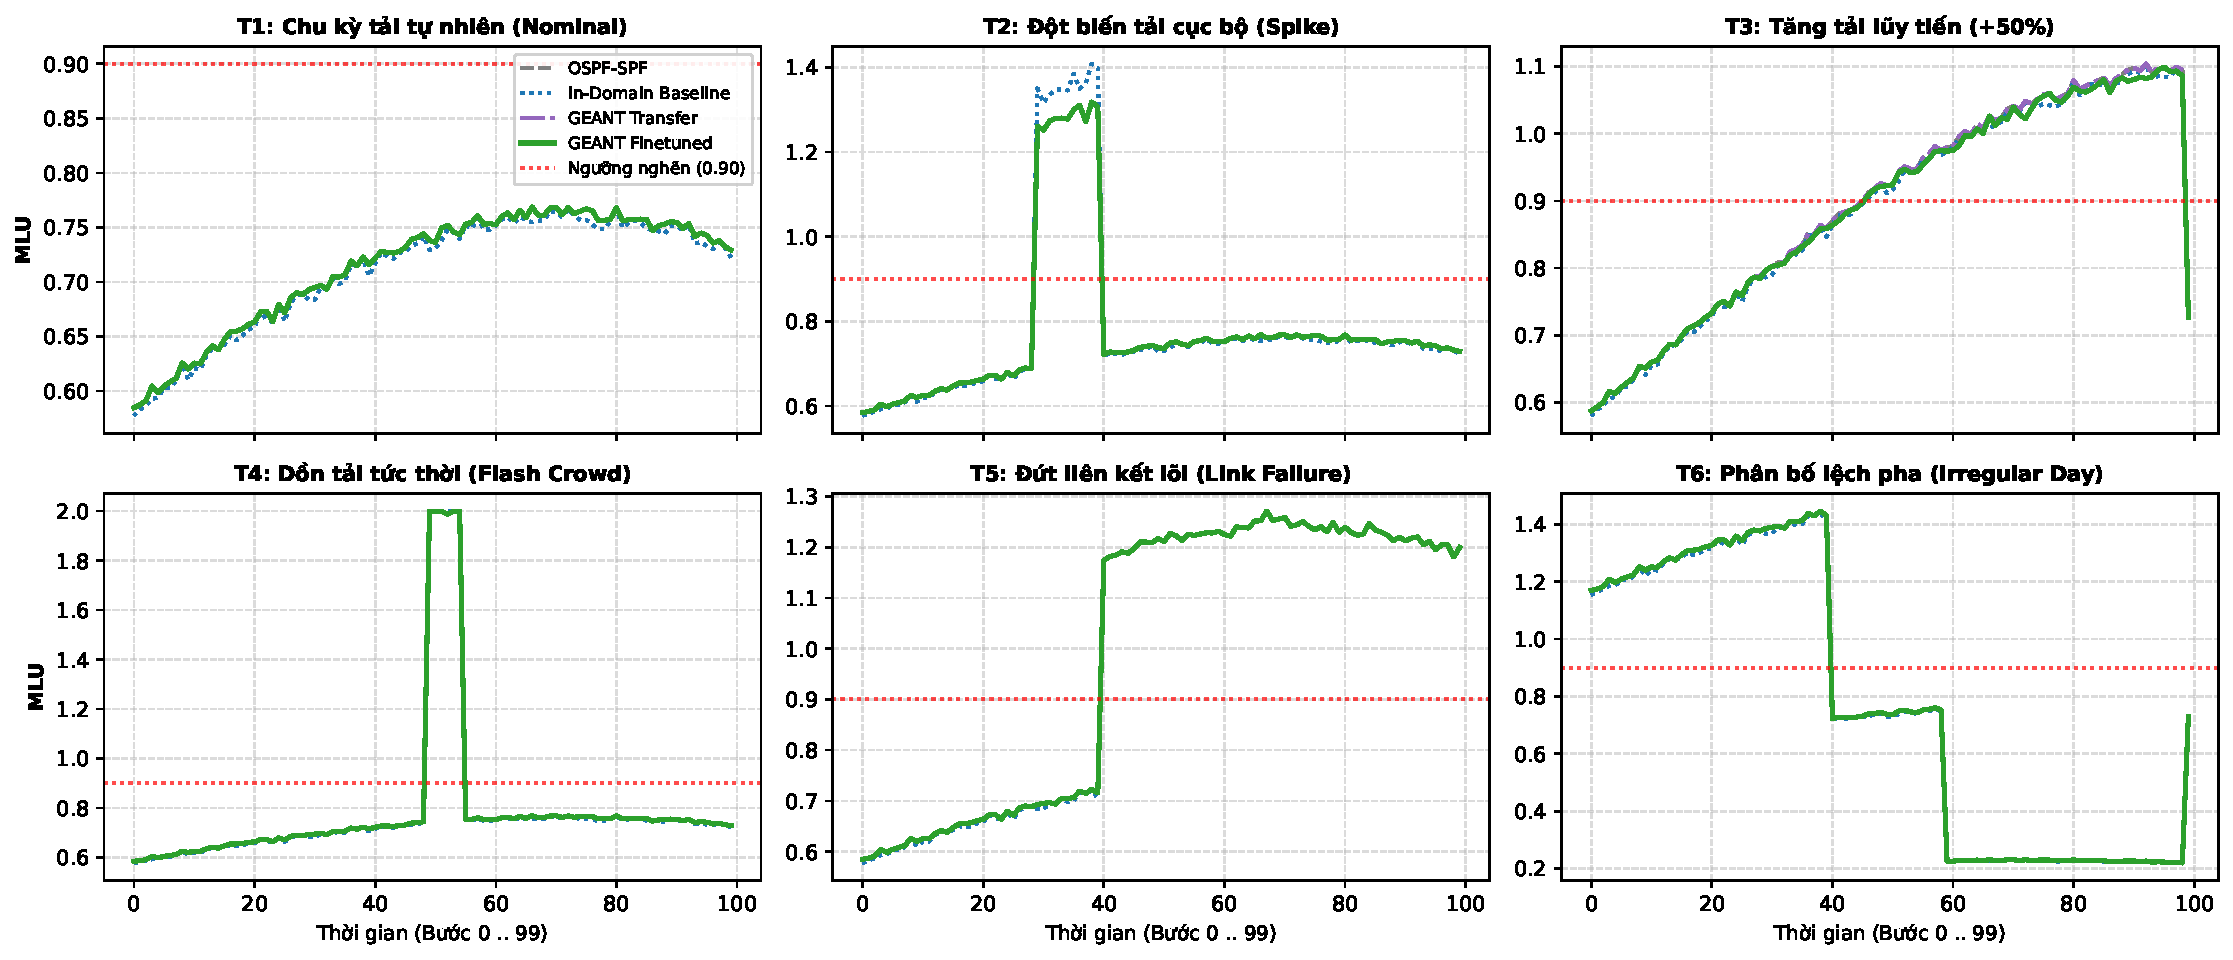
\includegraphics[width=\textwidth]{figures/overview_abilene_mlu.pdf}
        \caption{Mức sử dụng cực đại (MLU)}
    \end{subfigure}
    \vspace{0.15cm}
    \begin{subfigure}[b]{0.96\textwidth}
        \centering
        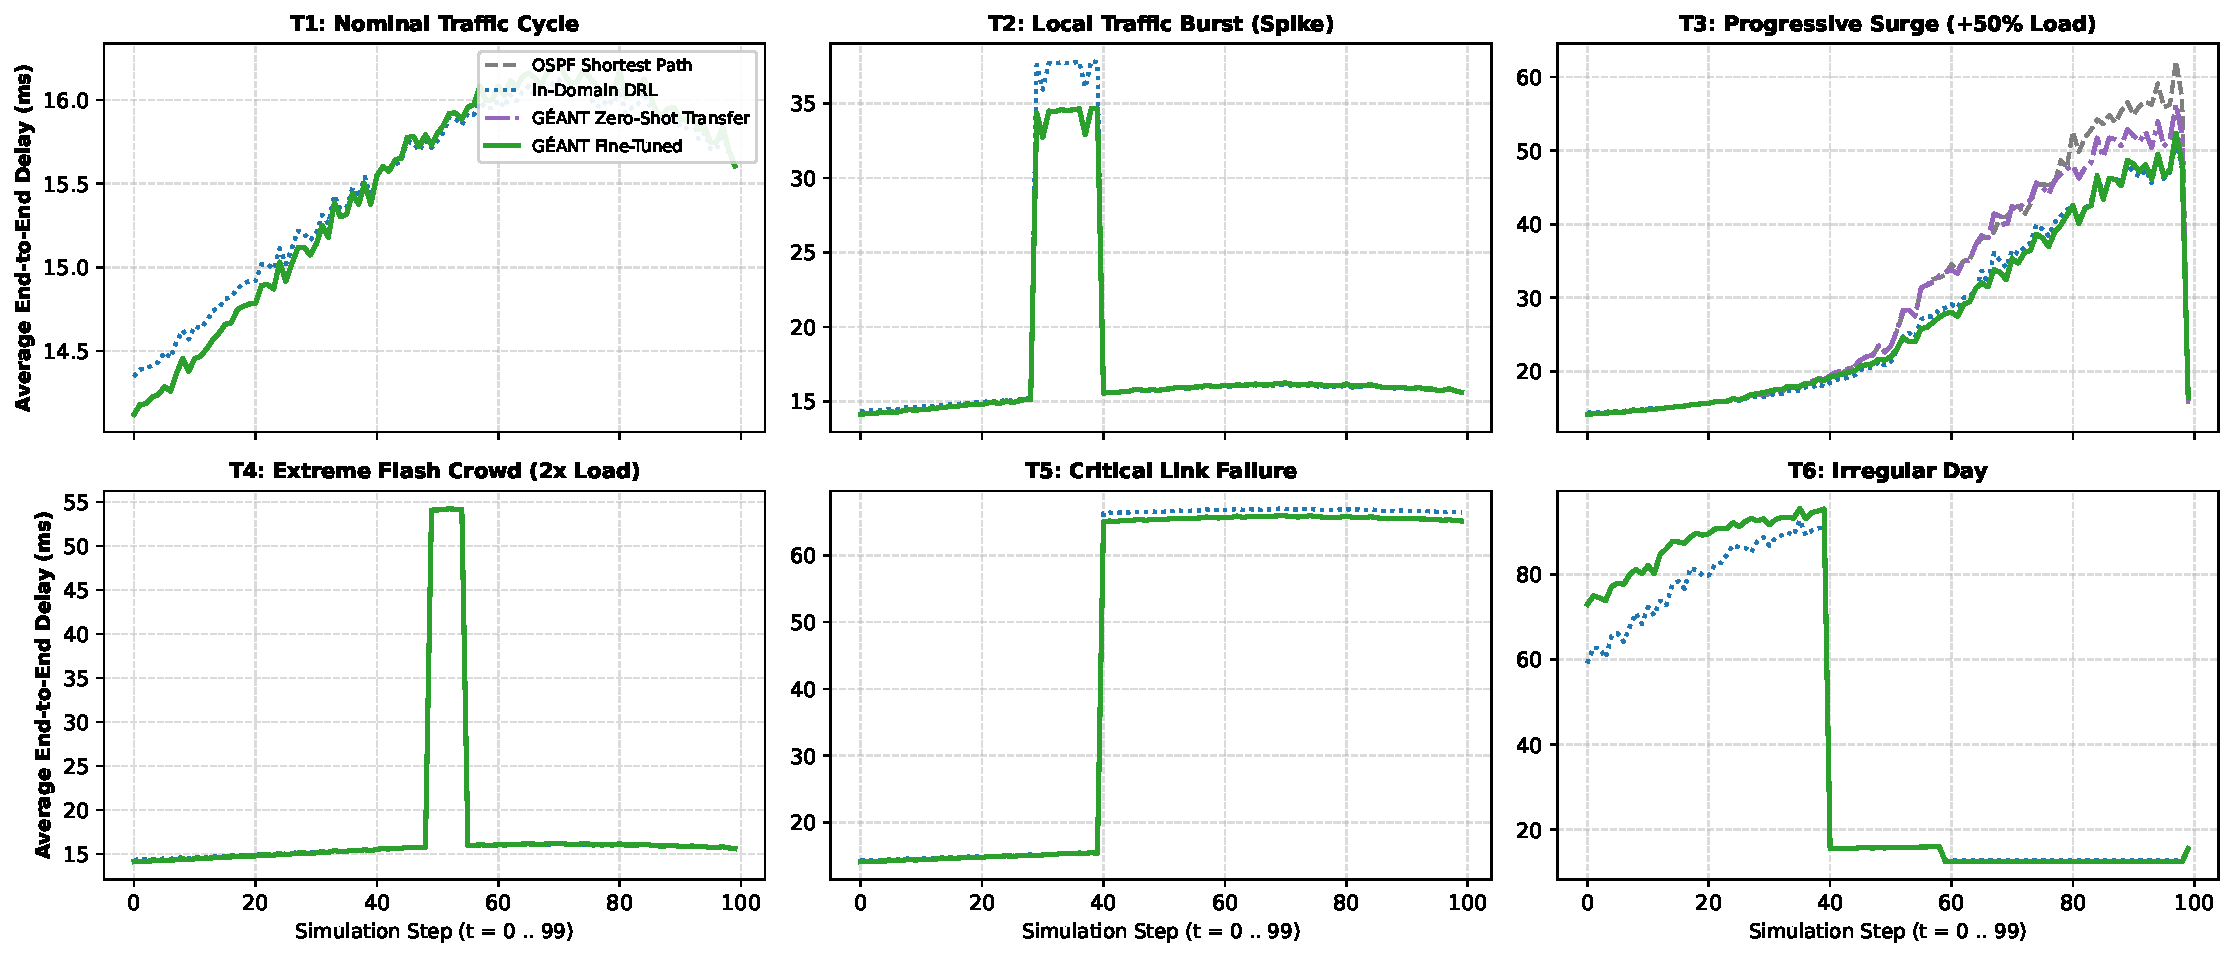
\includegraphics[width=\textwidth]{figures/overview_abilene_delay.pdf}
        \caption{Độ trễ trung bình (ms)}
    \end{subfigure}
    \vspace{0.15cm}
    \begin{subfigure}[b]{0.96\textwidth}
        \centering
        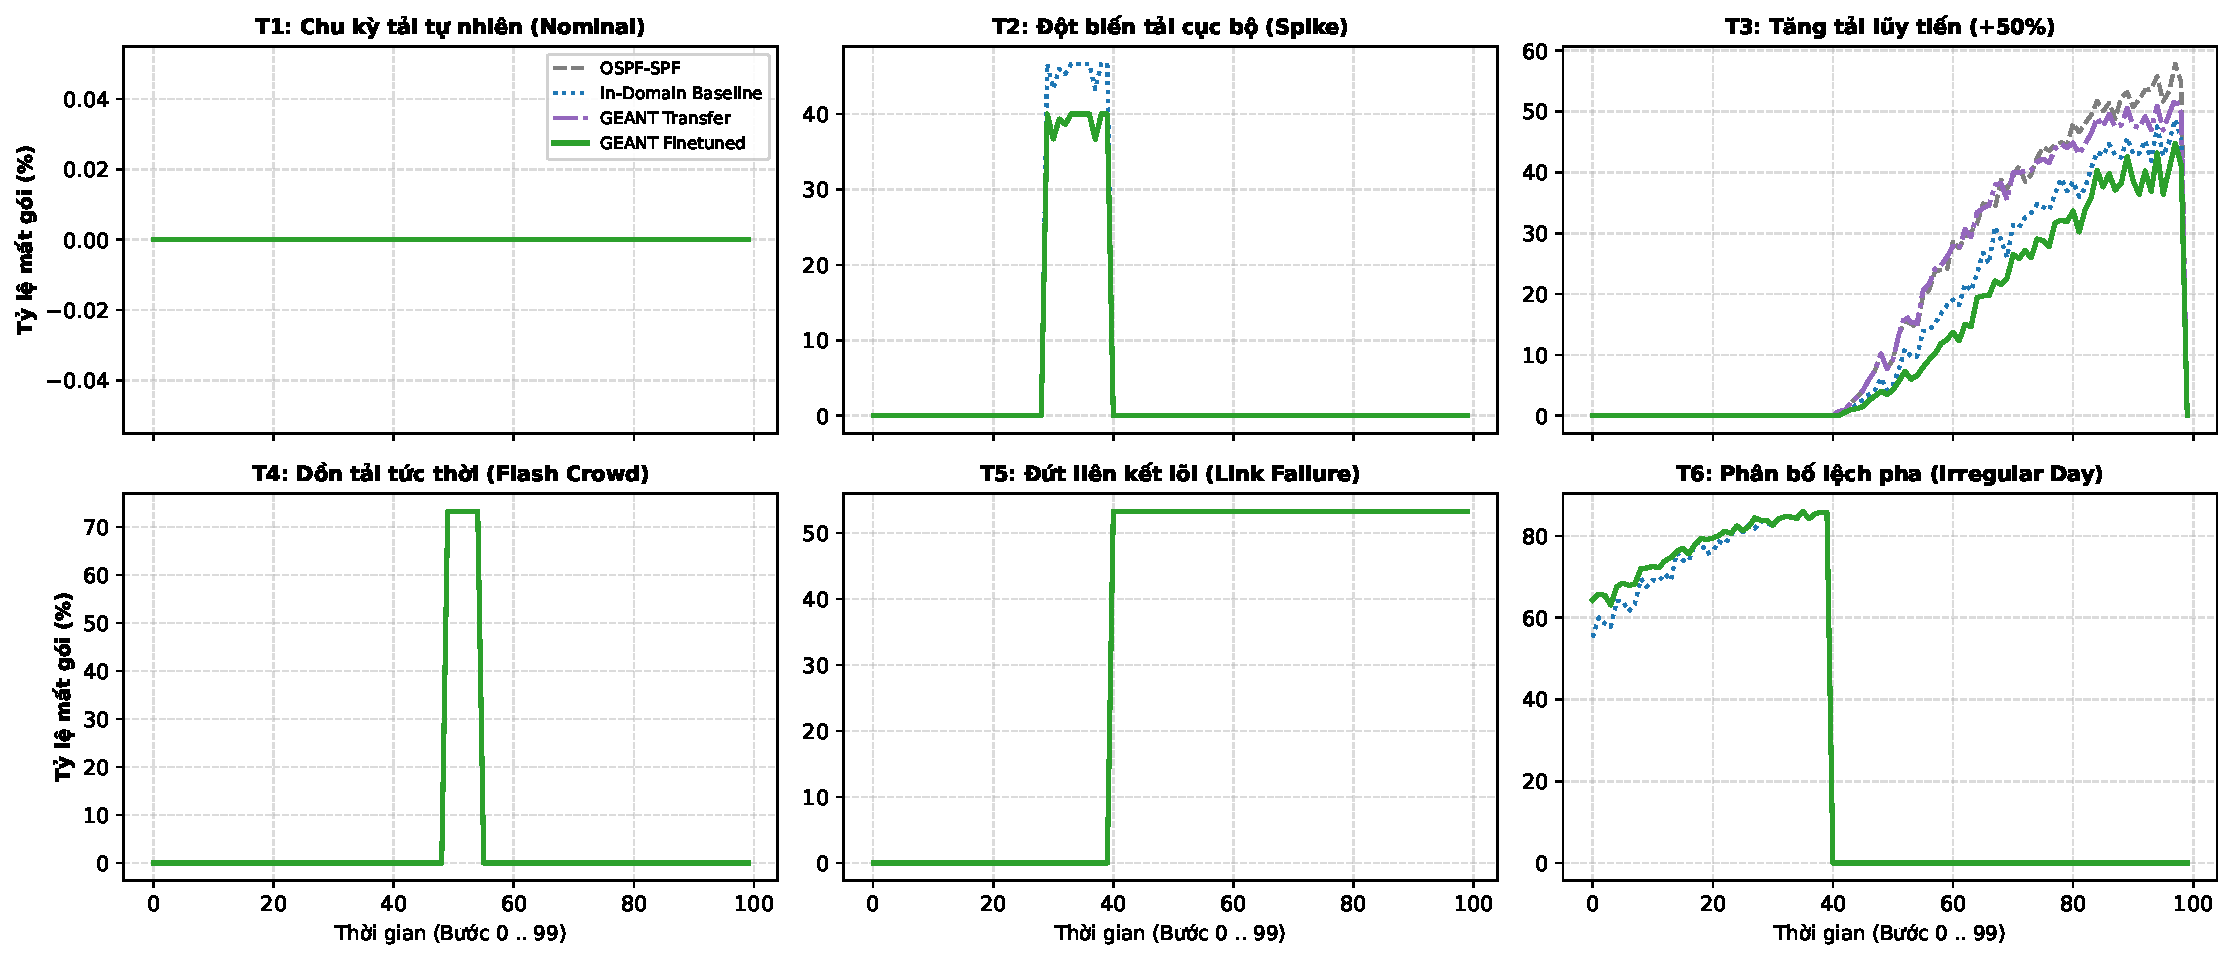
\includegraphics[width=\textwidth]{figures/overview_abilene_loss.pdf}
        \caption{Tỷ lệ mất gói (\%)}
    \end{subfigure}
    \caption{\textit{Toàn cảnh 6 kịch bản trên mạng Abilene: Đối sánh giữa OSPF, In-Domain, GEANT Transfer và GEANT Finetune (Lưới 2x3 vector chuẩn).}}
    \label{fig:abilene_all}
\end{figure}

\clearpage

Hệ thống hiện có thể chạy hoàn chỉnh pipeline thử nghiệm và đánh giá tự động bằng script \texttt{run\_full\_pipeline.py} và \texttt{demo.py}, kết nối trực tiếp giữa môi trường mô phỏng, mô-đun FL và tác tử PPO, xuất đầy đủ dữ liệu CSV và đồ thị trực quan so sánh với OSPF.
\section{Công việc đang thực hiện}

Hiện tại, nhóm đang tập trung thực hiện các nội dung công việc sau:
\begin{itemize}[leftmargin=1.5em, itemsep=0.3ex]
    \item \textbf{Hoàn thiện văn bản Báo cáo Khóa luận tốt nghiệp chi tiết:} Hệ thống hóa toàn bộ cơ sở lý thuyết, kiến trúc hệ thống, thuật toán FL/RL và phân tích chuyên sâu các bảng số liệu, biểu đồ thực nghiệm trên cả 3 mạng vào các chương theo quy định của Trường.
    \item \textbf{Mở rộng kiểm thử thực nghiệm trên Mininet thời gian thực:} Tiến hành đo đạc đối sánh với các luồng truyền video streaming UDP và lưu lượng TCP tải nặng để quan sát trực quan phản xạ tái định tuyến của Ryu Controller.
    \item \textbf{Chuẩn bị slide báo cáo và kịch bản demo:} Xây dựng bài thuyết trình bảo vệ khóa luận và hoàn thiện kịch bản demo trực quan trên giao diện giám sát mạng SDN.
\end{itemize}
\section{Công việc dự kiến tiếp theo}

Trong giai đoạn tiếp theo, các công việc dự kiến gồm:
\begin{itemize}[leftmargin=1.5em, itemsep=0.3ex]
    \item \textbf{Hoàn tất toàn bộ bản thảo khóa luận tốt nghiệp} và nộp phản biện theo đúng tiến độ của Khoa.
    \item \textbf{Báo cáo thử nghiệm và chạy demo kiểm tra} trước Giảng viên hướng dẫn để tiếp thu góp ý hoàn thiện.
    \item \textbf{Đóng gói mã nguồn}, cập nhật tài liệu hướng dẫn cài đặt và triển khai chi tiết trên GitHub phục vụ hội đồng chấm khóa luận.
\end{itemize}

\vspace{0.4cm}
Mã nguồn code: \url{https://github.com/Ragingsnake/ryu-fl-rl-traffic-controller}

\end{document}
